\documentclass{acm_proc_article-sp}
\usepackage[english]{babel}
\usepackage[utf8]{inputenc}
\usepackage{enumitem}
\usepackage{minted}
\usepackage{float}
\usepackage{listings}
%\usepackage{fixltx2e}
\usepackage{graphicx,url}
\usepackage[hidelinks,breaklinks]{hyperref}
\PassOptionsToPackage{hyphens}{url}

\usepackage{fancyhdr}
\usepackage{lastpage}
\pagestyle{fancy}
\fancyhf{}
\renewcommand{\headrulewidth}{0pt}
\renewcommand{\footrulewidth}{1pt}
\pagenumbering{arabic}
\fancyfoot[LE,RO]{\thepage}

\newcommand{\subparagraph}{}
\usepackage{titlesec}
\setcounter{secnumdepth}{4}


\addto\captionsenglish{\renewcommand{\bibname}{REFERENCES}}
\addto\captionsenglish{\renewcommand{\refname}{REFERENCES}}

\titleformat{\paragraph}
{\normalfont\normalsize\bfseries}{\theparagraph}{1em}{}
\titlespacing*{\paragraph}
{0pt}{3.25ex plus 1ex minus .2ex}{1.5ex plus .2ex}


\begin{document}
\thispagestyle{empty}

\title{LibsensorPy: An Extendable Python Library To Manipulate Sensors Coupled To The Raspberry Pi}

\numberofauthors{2} 
\author{
% 1st. author
\alignauthor
Edivaldo M. F. de Jesus Jr\titlenote{Student from the course of Analysis and Systems Development (ADS).}\\
       \affaddr{Instituto Federal da Bahia}\\
       \affaddr{Rua Em\'idio dos Santos, S/N}\\
       \affaddr{Barbalho, Salvador Bahia}\\
       \email{juniorug@gmail.com}
% 2nd. author
\alignauthor
Manoel C. M. Neto\titlenote{Ph.D. in Computer Science, Professor and Researcher from the course of Analysis and Systems Development.}\\
       \affaddr{Instituto Federal da Bahia}\\
       \affaddr{Rua Em\'idio dos Santos, S/N}\\
       \affaddr{Barbalho, Salvador Bahia}\\
       \email{manoelnetom@ifba.edu.br}
}

\date{13 April 2015}

\maketitle
\begin{abstract}

The convergence of radio technologies, microprocessors and personal digital electronic devices is leading to the concept of ubiquitous computing in which intelligent, mobile and stationary devices, coordinate with each other to provide for users immediate and universal access to new services transparently, aimed at increasing human capabilities. This work is intended to be inserted in this context and aims to define, implement and validate the design and implementation of an extensible Python library for manipulating sensors/actuators coupled to the Raspberry Pi using the raspberry-GPIO-python module. The library, called libsensorPy, uses Abstract Factory pattern to ensure that sensors/actuators and events from the same family being used in conjunction with guaranteed way. On other platforms, such as Arduino, APIs provide libraries that encapsulate the complexity of implementation and offer only the interface to use. These libraries do not yet exist formally for those who want to use Python as development language applied to the Raspberry Pi. This project also presents the results obtained using some of the implemented sensors, system modeling and results described and analyzed.

\end{abstract}
\keywords{Ubiquitous Computing, Internet of Things, Raspberry Pi, Sensor, Python.} 

\section*{Introduction}
\label{sec:Introduction}
The Ubiquitous Computing (UbiComp) in its several ramifications and applications, is treated by many as the twenty-first century's new paradigm of computing. UbiComp is the area of computing that studies the coupling of physical world to the world of information and provides an abundance of services and applications, allowing users, machines, data and objects of physical space interact with each other seamlessly. The theme is considered one of the great challenges of research in Computer Science by the National Science Foundation (NSF)\cite{NSF} and is also present in the report \textit{Grandes Desafios da Pesquisa em Computação no Brasil 2006-2016}\cite{carvalho2006grandes}, published by the SBC (Brazilian Computer Society - \textit{Sociedade Brasileira de Computa{\c{c}}{\~a}o}).
\newline
\newline
Researches on ubiquitous computing are being held on topics such as: basic access to any wireless device, mobility support on the network in a transparent manner, safety, context treatment, efficient use of energy, presentation of multimedia content, among others. This work is focused on building intelligent interactive environments. In these environments, the fundamental idea is to create ways to avoid the user need to go to the computer/device, allowing many of these working at a distance. The use of platforms to integrate devices that make up these environments is one of the key points to create it. Currently there are some options to fill this gap. This text emphasizes one: the project Raspberry Pi \cite{Trapp,wirth2014making}.
\newline
\newline
Raspberry Pi(RPi) is a widely used platform for professionals who are interested in the field of ubiquitous applications. It provides basic interfaces for creating small projects and/or for those who must be fed by battery. The platform allows the use high-level programming languages that are quite widespread as C/C ++, Python and Java. The Raspberry allows the development of a range of projects. For example, home automation (turn on and off electrical devices, remote control for TV, Air-conditioners, etc.), eBook and Audiobook readers and so on.
\newline
\newline
A brief search about how to access the Raspberry Pi bus will bring  a lot of papers in Python. Which incidentally, introduce the acronym of the device name (Pi from Python). However, any library that abstracts the details of wiring a sensor or actuator to the Raspberry allowing the user takes care just in read the data already processed and/or converted will not be found.
\newline
\newline
The developer must have a degree of experience that can be considered basic to a professional, but advanced for those who are not.
\newline
\newline 
This paper is structured as follow:

Section~\ref{sec:theoreticalBackground} present several technologies involved in the preparation of this article, aimed to introduce important concepts of Computer area in which the context of this project is inserted. Section~\ref{sec:relatedWork} shows correlated works. Section~\ref{sec:proposedModel} presents details of the executed implementation. The last section presents the conclusions.




\section{THEORETICAL BACKGROUND}
\label{sec:theoreticalBackground}
In this section the main concepts studied are presented, which provided subsidies for the development of the proposed project.

\subsection{General Context}
The term Ubiquitous Computing was first defined by Mark Weiser \cite{weiser1991} in the late 80. At this time, Weiser predicted an increasing in functionality and availability of computing services to end users and, on the other hand, he predicted a decreased visibility of these services. For Weiser, the computing would not be exclusive of a PC. He believed that in the future there would be several different devices connected to each other. At a time when users were using PCs (desktops) and that knowledge needed to operate a computer,  Weiser bet on a future where the focus of the users would be the task itself, and not the tool used. In this way, they would use computers without realizing or require specific technical knowledge. \cite{weiser1994world}
\newline
\newline

The passage of time has shown that Weiser's bet was right. For Weiser, \cite{weiser1997coming} evolution of computing has gone through two ages to reach to ubiquitous computing. The first was called the age of mainframe, where many people shared the same computer. The second era was the PC, where each computer was used by one person. Currently, the evolution of distributed information systems, the network connections type options'  expansion, mobile computing and various types of applications on non-conventional computing devices, are just some of the examples that can confirm: Ubiquitous Computing (the third age) is already a reality. Figure~\ref{fig:era} shows a chart with the ages of computing.
\newline
\newline

\begin{figure}[h]
\centering
    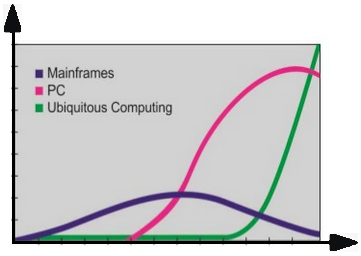
\includegraphics[width=0.4\textwidth,natwidth=610,natheight=642]{pictures/era.png}
    \caption{Ages of Computing}
    \label{fig:era}
\end{figure}

Terms such as ubiquitous computing, pervasive computing, nomadic computing, invisible computing, mobile computing and many others, have been used often interchangeably, although they differ conceptually and employing different organization of ideas and management of computer services. Insofar as each area progresses, these concepts will be better understood and its definitions will become clearer. This section presents the key concepts needed to understand the UbiComp besides presenting some project examples in the literature.

\subsection{Mobile Computing}
Mobile computing is based on the ability of a user to load or move (physically) computer services wherever it moves. In this context, the computer becomes an ever-present device that expands the ability of a user to use the services it offers, regardless of their location. Combined with the ability to access network, mobile computing has transformed the computing an activity that can be taken almost anywhere \cite{netodesenvolvimento}.
\newline
\newline
An important conceptual limitation of mobile computing is that the computational model used in most applications does not change while users are moving. It means that a device is not able to obtain information on the physical context in which computation occurs, and consequently also can not adapt to the new context correctly. A solution to accommodate the changing context would pass to users the responsibility to monitor and manually configure an application / device to the extent that it moves. However, this solution is not well accepted by most users. This limitation was one of the inspirations for pervasive computing .

\subsection{Pervasive Computing}
The concept of pervasive computing implies that the computer is embedded invisibly in the environment to the user \cite{krumm2009}. In this conception, the computer has the ability to: i) obtain environmental information in which it is embedded and ii) use it to build dynamically computational models that allow controlling, configuring and tuning application to better suit the needs of a device or user. For this to be possible, the key point is the ability of computers be able to act as "smart" in the environment where users move. This environment is usually populated by computational sensors and services.

\subsection{Ubiquitous Computing}
Ubiquitous is an adjective originated from Latin (\textit{ubiquu}) which means "that is at the same time everywhere". As can be seen in figure~\ref{fig:ubiq}, the UbiComp can be defined as a computer area positioned between Mobile Computing and Pervasive Computing \cite{de2003computaccao,krumm2009}. Ubiquitous computing benefits from the advances in mobile and pervasive computing and arises from the need to integrate mobility with the functionality of pervasive computing. The term ubiquitous computing will be used here as a junction of pervasive computing and mobile computing. The justification to perform a distinction of these terms is a device that is embedded in an environment, not necessarily is mobile.
\begin{figure}[h]
\centering
    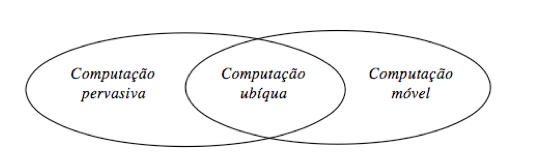
\includegraphics[width=0.4\textwidth,natwidth=610,natheight=642]{pictures/ubiq.png}
    \caption{Ubiquitous Computing: intersection between pervasive and mobile computing}
    \label{fig:ubiq}
\end{figure}
\newline
\newline
Research in ubiquitous computing approach about technologies and infrastructure that enable deployment of ubiquitous applications through a number of issues including the following:

\begin{itemize}
\item How to design hardware and operating systems for sensor platforms?
\item How to allow devices to find each other and to use their services?
\item How to allow systems involving limited processing resources and energy, to work well?
\end{itemize}

Generally, ubiquitous applications receive sensor data from other service providers devices, manage user actions, provide support mobility and use context information to perform tasks \cite{doesntfit}. A ubiquitous system itself has a set of requirements, peculiarities and challenges that influence design, implementation, deployment and evaluation of its project \cite{krumm2009}. These are cornerstones of UbiComp and quite different from those used in development of systems for PC's. Among these points, can be cited as an example \cite{krumm2009}:

\begin{enumerate}
\item Resource-Constrained Devices; 	
\item Volatile Execution Environments; 	
\item Heterogeneous Execution Environments;
\item Fluctuating Usage Environments;
\item Invisible Computing;
\item Security and Privacy;
\end{enumerate}

\subsection{Internet of Things}
The Internet of Things (IoT) is a multidisciplinary field, covering a wide range of subjects, from purely technical issues (e.g., routing protocols, semantic queries) to a mixture of technical and social problems (security, privacy, usability) as well as social and business topics. The existing Internet of things applications are potentially diverse. Environmental and personal health monitoring, monitoring and control of industrial processes including agriculture, smart spaces, and smart cities are just some of the examples of IoT applications \cite{krishnakumarframework}.
\newline
\newline
The connection of physical things to the Internet makes it possible to access remote sensor data and to control physical world from a distance. The mash-up of captured data with data retrieved from other sources, e.g., with data that is contained in the Web, gives rise to new synergistic services that go beyond services that can be provided by an isolated embedded system. The Internet of Things is based on this vision. A smart object, which is the building block of the Internet of Things, is just another name for an embedded system that is connected to the Internet \cite{Kopetz:1997}.
\newline
\newline
Everyday physical things that are enhanced by a small electronic device to provide local intelligence and connectivity to the cyberspace established by the Internet. The small electronic device, a \textit{computational component} that is attached to a \textit{physical thing}, bridges the gap between the physical world and the information world. A \textit{smart object} is thus a \textit{cyber-physical system} or an \textit{embedded system} consisting of a \textit{thing} (the physical entity) and a \textit{component} (the computer) that processes sensor data and supports a wireless communication link to the Internet \cite{Kopetz:1997}.

\subsection{Hardware}
One fundamental requirement for developing ubiquitous systems is the use of hardware such as sensors, microcontrollers, communication devices (network cards, Bluetooth, etc.) and storage, among others. For example, sensors allow transform use of interactive environments from more transparent interfaces. Currently, there are some platforms that allow insert and control various types of sensors, using of communication interfaces and storage units. This section presents and details the main hardware devices available for development of ubiquitous systems.

\subsubsection{Sensors and Actuators}
Sensors are devices that allow us to capture information from the environment in which they are inserted, such as temperature, pressure, presence, humidity, smoke detector, light intensity, among others. In general, sensors work transforming parts of a physical quantity into an electrical signal, which in turn can be interpreted by electronic devices \cite{borges2010automaccao}. In other words, sensors are components that allow an electronic device to interact with real world.
\newline
\newline
According to \cite{borges2010automaccao}, when sensors operate directly, transforming one form of energy into another are called transducers. Sensors where operations occur indirectly alter their properties, such as resistance, capacitance or inductance, under the action of physical grandeur so that this change is roughly proportional. For example, the light sensor LDR (Light-dependent resistors) vary inversely its resistance the amount of light falling on it. Thus, when there is a large amount of light falling on the sensor, they have a very low resistance and this allows the flow of electric current increases, whereas when there is little light, they have a high resistance and prevent current flow.
\newline
\newline
An actuator as well as a sensor is a transducer that converts one form of energy into another, and can also do the opposite \cite{borges2010automaccao}. In other words, rather than just  transform parts of a physical quantity into an electrical signal, it can transform an electrical signal into a physical quantity such as motion, magnetism, heat, among others. For example, relays are electromechanical devices that work with small power, but are able to control external circuits that involve high currents. They are basically composed of a coil and a set of contacts. When a current flows through the coil it creates a magnetic field that attracts and closes the contacts, remaining as long as power supply in the coil. As a result, it allows the passage of energy through the relay.

\subsubsection{Arduino}
Arduino was created in 2005 by Massimo Banzi and David Mellis in Italy with the goal of use as an electronic learning tool and programming for design students, so that they would use in art projects, interactivity and robotics. Electronic learning was expensive: a microcontroller was costing 100 euros. So they decided to make their own board. Sought employees and thus created an efficient technology, accessible and compatible with Windows, Mac and Linux \cite{netodesenvolvimento}.
\newline
\newline
Arduino is a platform that popularizes the concept of free hardware. In the book Getting Started with Arduino, Massimo Banzi describes the Arduino as a physical open-source computing platform based on a simple board with input/output pins that implements the Processing language. Constituted by a microcontroller, this small but powerful board can be easily programmed via a Universal Serial Bus interface (USB) and able to build electronic devices and interesting systems.
\newline
\newline
Working with construction of a hardware requires much time and effort, because is necessary to create new circuits, use various components such as resistors and capacitors and many welds. Using Arduino board abstracts much of this construction process, making it simpler, allowing people from different fields of knowledge being able to build their projects. The platform is widely used worldwide for offering advantages such as:


\begin{itemize}
\item A multi-platform environment that can run all major operating systems such as Windows, Linux and MacOS.
\item An open-source hardware, i.e., the circuit design is available so that if someone is interested in creating their own card, just buy the necessary components.		
\item Hardware cost is low.					
\item Can be programmable via a USB cable instead of a serial port. Remember that today's computers do not have serial ports.	
\item It has a development environment with intuitive interface for easy use.
\end{itemize}

The fact that both the hardware and the Arduino software be developed in an open, patent-free, allows its projects to be recreated in different ways. The adoption of open hardware concept motivates those who create projects to contribute with functions and libraries for the Arduino. Is knowledge about knowledge, the same principle of free software.
\newline
\newline
Note that there is not necessary advanced knowledge in electronics to use the platform. But for those who are interested in deepening the knowledge in this area, there are several available materials that can help, for example, in \cite{Eletronica}.

\subsubsection{BeagleBone}
The BeagleBoard is a low-power open-source hardware single-board computer produced by Texas Instruments in association with Digi-Key and Newark element14. The BeagleBone Black was also designed with open source software development in mind, and as a way of demonstrating the Texas Instrument's OMAP3530 system-on-a-chip\cite{coley2009take}. The board was developed by a small team of engineers as an educational board that could be used in colleges around the world to teach open source hardware and software capabilities. Sold to the public under the Creative Commons share-alike license, the board was designed using Cadence OrCAD for schematics and Cadence Allegro for PCB manufacturing; no simulation software was used.
\newline
\newline
BeagleBone is an \$89 Manufacturer suggested retail price (MSRP) credit-card-sized Linux computer that connects to the Internet and runs software such as Android 4.0 and Ubuntu. With plenty of I/O and processing power for real-time analysis provided by an AM335x 720MHz ARM\textregistered\, processor, BeagleBone can be complemented with cape plug-in boards to augment functionality.

\subsubsection{Raspberry Pi}
Raspberry Pi is a small computer, approximately with the size of a credit card. It can be used to do many things that are done by a common personal computer\cite{raspberryfoundation}. In addition, it can also be used in electronic projects because it has a hardware interface: The general purpose input/output port (GPIO). The Raspberry Pi Foundation, creator of the project, is an educational charity headquartered in the UK and aims to help and encourage the teaching of computer science in schools.
\newline
\newline
This computer came up with intention of reconnecting children and youth in computer programming and stimulate the creation of new projects so there is not only the consumption of the technology created by the market. While in the 1990s there was a growth in the number of children and youth who developed programming skills, starting in the 2000s, this number started to decline \cite{raspberryAbout}.
\newline
\newline
With the realization that, year by year, students were moving away from programming and reducing the development of skills in computer science. The researchers Eben Upton, Rob Mullins, Jack Lang and Alan Mycrof, from the Computer Laboratory of University of Cambridge had the idea of creating a platform that would allow to reconcile the programming students  and handling computers\cite{dennis2013raspberry}. From 2006 to 2008, early versions of what is now the Raspberry Pi was developed. From 2008, with the expansion and emphasis on mobile devices, the devices are becoming more efficient and cheaper which enabled the launch of the Raspberry Pi model B to the public in February 2012 for \$ 35.
\newline
\newline
The proposal of the Raspberry Pi is therefore be a low-cost computer, with the ability to interact with the outside world through the sensor coupling. As seen previously, it was thought to be used in the educational environment, in order to assist and encourage the teaching of programming and help understand the operation of computers. However, the Raspberry Pi has been used by people of all ages and interests in various projects, for example, projects involving automation, sensing and robotics, games, multimedia, networks and servers.
\newline
\newline
Currently there are three  Raspberry Pi models: The model A, which costs \$ 25 and the B and B+ models, which costs \$ 35. As for the price, there is not much difference between hardware models. The main differences are the amount of USB ports (1, 2 and 4 in the models A, B and B +, respectively), the Ethernet port (model A does not have) and ram (256MB on the model A against 512 for the others).
\begin{figure}[h]
\centering
    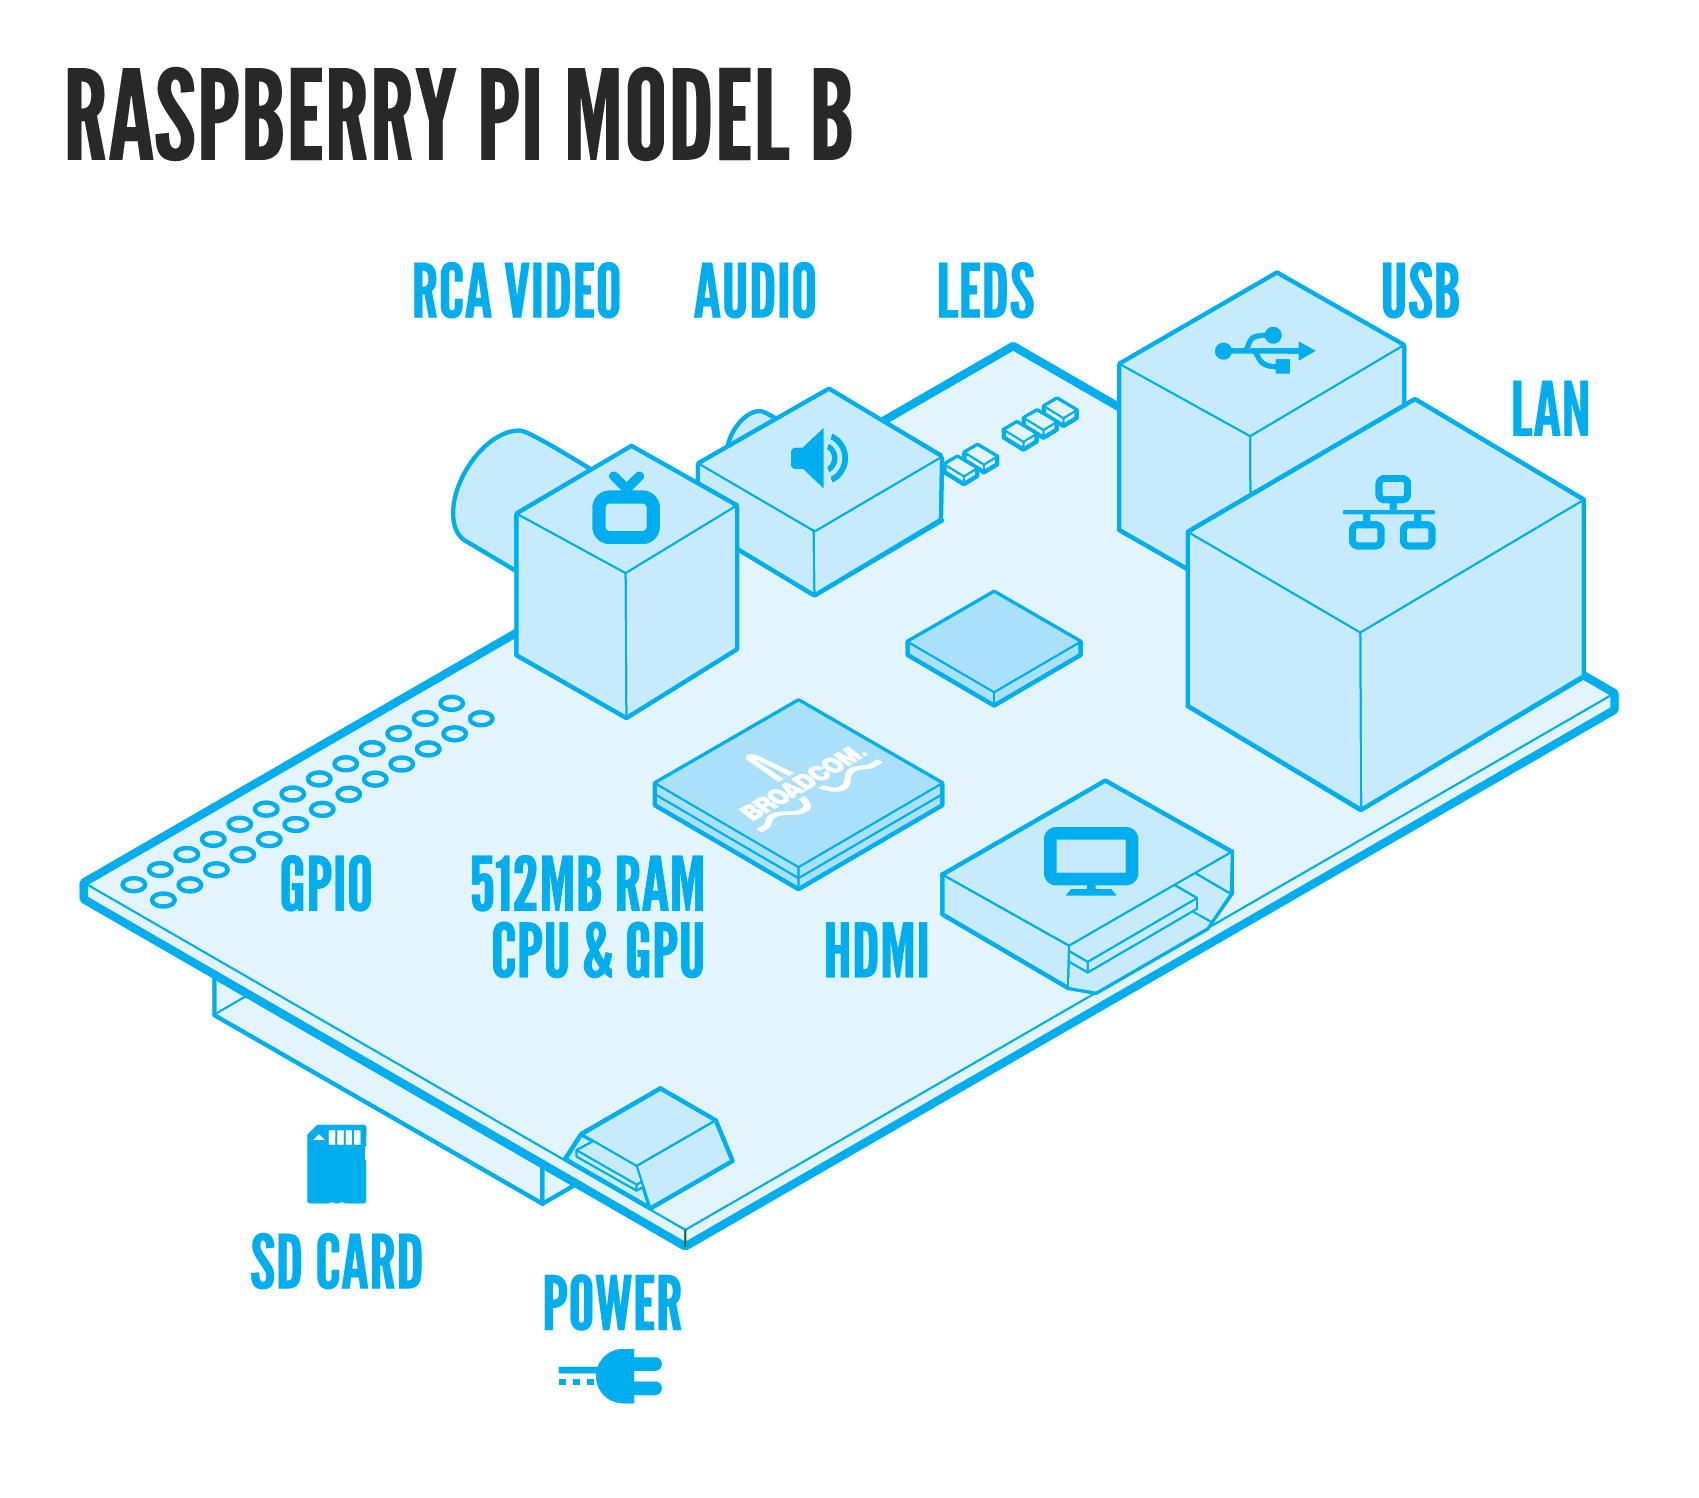
\includegraphics[width=0.5\textwidth,natwidth=610,natheight=642]{pictures/RaspiModelB.png}
    \caption{Raspberry Pi Components, model B\protect\cite{raspberryFaq}}
    \label{fig:raspi}
\end{figure}

\paragraph{Features}
The original RPi is based on the Broadcom BCM2835 system on a chip (SoC)\cite{Broadcom}, which includes an ARM1176JZF-S 700 MHz processor, VideoCore IV GPU\cite{Brose}, and was originally shipped with 256 megabytes of RAM, later upgraded (models B and B+) to 512 MB\cite{raspOrg}. The system has Secure Digital (SD) (models A and B) or MicroSD (models A+ and B+) sockets for boot media and persistent storage\cite{Elinux}.
\newline
\newline
In 2014, the Raspberry Pi Foundation launched the Compute Module, which packages a BCM2835 with 512 MB RAM and an eMMC flash chip into a module for use as a part of embedded systems \cite{raspNewProduct}.
The Foundation provides Debian and Arch Linux ARM distributions for download. Tools are available for Python as the main programming language, with support for BBC BASIC (via RISC OS image or the Brandy Basic clone for Linux)\cite{Jaguar}, C, C++, Java, Perl and Ruby.
\newline
\newline
Some other features presents on RPI:
\begin{itemize}
\item Display Serial Interface Connector (DSI): This connector receives a flat-ribbon cable of 15 pins that can be used to communicate with an LCD or organic light-emitting diode (OLED) display screen;	
\item Camera Serial Interface(CSI) Connector: This port allows a camera module be directly coupled to the card;
\item P2 and P3 connectors: These two rows of connectors are JTAG connectors for test to Broadcom chip (P2) and LAN9512 network (P3). Due to the proprietary nature of Broadcom chipset, these connectors are unlikely to be of much used;
\item Pin Protection: Most of the pins in the header go directly to the Broadcom chip. Carefully design the components what can be attached to the pins is very important as there is a risk of permanently damage the RPi. Short circuits and wiring mistakes could also shatter the board, so double check everything. A multimeter is probably going to help a lot here as the developer can double check wiring before connect to the RPi.
\end{itemize}

\paragraph{Power Supply}
The device is powered by 5v micro USB. Exactly how much current (mA) the Raspberry Pi requires is dependent on what the project hook up to it. Purchasing a 1.2A (1200mA) power supply from a reputable retailer will provide to the user with ample power to run the Raspberry Pi for most applications, though may want to get a 2.5A (2500mA) if necessary to use all 4 USB ports on the Model B without using an external powered USB hub.
\newline
\newline
The power requirements of the Raspberry Pi increase as much as are used the various interfaces on the Raspberry Pi. The GPIO pins can draw 50mA safely (that is 50mA distributed across all the pins! An individual GPIO pin can only safely draw 16mA), the HDMI port uses 50mA, the camera module requires 250mA, and keyboards and mice can take as little as 100mA or over 1000mA. Check the power rating of the devices  what are planed to connect to the Pi and a power supply must be purchased accordingly.

\paragraph{Processor}
The System on a chip(SoC) used in the first generation Raspberry Pi is somewhat equivalent to the chip used in older smartphones (such as iPhone / 3G / 3GS). The Raspberry Pi is based on the Broadcom BCM2835 system on a chip (SoC)\cite{Broadcom}, which includes an 700 MHz ARM1176JZF-S processor, VideoCore IV GPU\cite{Brose}, and RAM. It has a Level 2 cache of 128 KB, used primarily by the GPU. The SoC is stacked underneath the RAM chip, so only its edge is visible.

\paragraph{General Purpose Input/Output}
Another important aspect of hardware from Raspberry is the group of GPIO pins. These pins are programmable ports to input and output data used to provide an interface between the board and peripherals, microcontrollers/microprocessors, sensors, actuators, etc. The GPIO interface is fundamental for building intelligent interactive environments and it is the interface between the Raspberry and the real world. In simple terms, the GPIO pins can be considered as switches that can be turned on/off.
\newline
\newline
Similarly to the Arduino, besides the GPIO, the Raspberry also supports PWM (Pulse Width Modulation), UART (Universal asynchronous receiver/transmitter) and SPI (Serial Peripheral Interface). Of the 26 pins available, 17 are reserved for GPIO and 8 are used for power and ground. Figure 2.6 shows the GPIO interface. These pins can be used via code written in a programming compatible language like Python, Scratch, Java, among others \cite{Brose}.
The GPIO pins are available on the PCB via a header and allow the Pi to interface with the real world.

\paragraph{Inputs and Outputs}
The number and options of input and output from a Raspberry Pi depend on the model used. Models RPi A+, B+ and 2B GPIO J8 have 40-pin as pinout. Models A and B have only the first 26 pins \cite{raspUsage}. In this paper will be presented only the pins available in the model B. The pins are divided into:

\begin{itemize}
\item Digital pin to input or output (programmable) - 17 pins;	
\item Analog input pins or digital input/output - 6 pins;
\item Power pins (gnd, 5V, 3.3V) - 9 pins;
\end{itemize}

The first item on the list are the useful pins. They are the ones that are available for a programmer use. Is through these pins that the Raspberry Pi is coupled to the sensors to capture environmental information. Among the 17 digital input/output pins there are 2 pins that match the serial communication module UART (Universal asynchronous receiver/transmitter). This module allows communication between a computer (for example) and the Raspberry Pi (see Special Pins section). All pins have more than one function, pins can be input or output, and the roles of each are defined in the code of possible programs that can be run on the RPi.

\paragraph{Digital Inputs}
All 17 programmable pins can be used as digital inputs. When a pin is programmed to function as digital input, can be used a command that, when executed, performs the "reading" of the voltage applied to it. Then, after running this command, the user  will know if the pin is in a "high" or "low" state (on or off).
\newline
\newline
From the electrical point of view, the program can tell if a pin is fed with 0 (zero) or 5 Volts. This function is usually used to identify whether a button is pressed or a sensor is capturing some environmental information. Note that the digital input function delivers only values 0 or 1 (no voltage or with voltage). How much voltage is being applied to the pin is not known.

\paragraph{Analog Inputs}
The Raspberry Pi does not have analog pins as Arduino, but is possible to use a traditional analog-to-digital converter(ADC) chip connecting to the RPi via SPI or I2C. For example the Microchip MCP3424 (I2C interface) which has 4 differential inputs. All ADC should work on the RPi, except that the timing is not as good as a microcontroller due to the available Linux versions not being true real-time. 

\paragraph{Digital outputs}
With a digital output is possible only two types of values (0 or 5 volts, 1 or 0, etc.). From a pin programmed as digital output is possible for example light up an LED, connecting a relay, trigger a motor, etc. All 17 digital outputs from the RPi can be programmed.

\paragraph{Special Pins}
RPi pins have some special characteristics which can be used from the software functions encoded by a software programmer. Are they:

\begin{itemize}

\item PWM - Pulse Width Modulation: Treated as analog output, this pin is actually a digital output that generates an alternating signal (between 0 and 1) where the time that the pin is in level 1 (on) is controlled. It can be used, for example, for engine speed control, or generate voltages with values controlled by the program. For the PWM communication may use pin 12 \cite{barr2001pulse};

\item UART - Universal asynchronous receiver/transmitter: One pin(TxD) is used to transmit and another(RxD) to receive data in serial asynchronous format. For example, to connect a data transmission module via bluetooth and allow communication with the Arduino remotely. Are reserved for UART pins 15 (RXD receives data) and 14 (TXD sends data) \cite{Uart};

\item SPI Port - Serial Peripheral Interface: These are pins that allow synchronous serial communication faster than UART. They allow for example to connect memory cards (SD) and many other things. Are used for this purpose the pins 19 as Master Output, Slave Input (MOSI), 21 as Master Input, Slave Output(MISO), 23 as Serial Clock(SCLK), 24 as Chip Select0(CE0) e 26 as Chip Select1(CE1) \cite{Spi};


\item I2C Bus - Inter-Integrated Circuit: The I2C bus allows multiple devices to be connected to the Raspberry Pi, each with a unique address, that can often be set by changing jumper settings on the module. To be able to see which devices are connected to the RPi is very useful as a way of making sure everything is working. Are used for this purpose pins 3 for Serial Data Line(SDA) and pin 5 for Serial Clock Line(SCL) \cite{I2c}.

\end{itemize}

\subsection{Software}
This section presents all software solutions which are involved with the proposed model.

\subsubsection{Operating systems}
Raspberry Pi primarily uses Linux-kernel-based operating systems. The ARM11 chip at the heart of the Pi (pre-Pi 2) is based on version 6 of the ARM. The current releases of several popular versions of Linux, including Ubuntu \cite{Gareth}, will not run on the ARM11. Run Windows on the original Raspberry Pi is not possible, though the new Raspberry Pi 2 will be able to run Windows 10\cite{Kevin}. The Raspberry Pi 2 currently only supports Ubuntu Snappy Core, Raspbian, OpenELEC and RISC OS.
\newline
\newline
The install manager for the Raspberry Pi is NOOBS. The operating systems included with NOOBS are:

\begin{itemize}

\item Archlinux ARM;
\item OpenELEC;
\item Pidora (Fedora Remix);
\item Puppy Linux;
\item Raspbmc and the XBMC open source digital media center;
\item RISC OS – The operating system of the first ARM-based computer;
\item Raspbian\footnote{Recommended for Raspberry Pi and used in this project} \cite{Raspbian} – Maintained independently of the Foundation; based on the ARM hard-float (armhf) Debian 7 'Wheezy' architecture port originally designed for ARMv7 and later processors (with Jazelle RCT/ ThumbEE, VFPv3, and NEON SIMD extensions), compiled for the more limited ARMv6 instruction set of the Raspberry Pi. A minimum size of 4 GB SD card is required. There is a Pi Store for exchanging programs\cite{PiStore}.
\begin{itemize}
\item The Raspbian Server Edition is a stripped version with fewer software packages bundled as compared to the usual desktop computer oriented Raspbian\cite{Yau,Raspbianwheezy}.
\item The Wayland display server protocol enable the efficient use of the GPU for hardware accelerated GUI drawing functions\cite{EbenUpton}. On 16 April 2014 a GUI shell for Weston called Maynard was released.
\item PiBang Linux is derived from Raspbian\cite{Pibanglinux}.
\item Raspbian for Robots\cite{DexterIndustries} - A fork of Raspbian for robotics projects with LEGO, Grove, and Arduino.
\end{itemize}

\end{itemize}

A list of other operating systems that can be installed on Raspberry Pi but are not included with NOOBS can be found in the appendix~\ref{sec:RPiOS}\footnote{\url{http://en.wikipedia.org/wiki/Raspberry_Pi\#cite_note-RaspbianServerEdition-78}}.


\subsubsection{WiringPi}
WiringPi is a library for access to GPIO interface written in C. Its use can be performed with C, C ++, or other programming languages through wrappers \cite{wiring}. Wrapper is an outer layer that extends WiringPi and can be implemented in different programming languages. This will allow the programmer to carry out projects not only in C or C ++, but also in language implemented by the wrapper. There are wrappers being developed in various languages such as Java, Ruby and Python. This last will be used in this paper from the wrapper raspberry-gpio-python.

\subsubsection{Python}
Python is considered a very high level language because its syntax is simple and its dynamic typing, besides being interpreted, which makes it great for scripting and robust for various paradigms including object orientation. With all these benefits of language, Python still surprises to be an open source software being available for all major operating systems\cite{dearduino}.

\subsubsection{GPIO in Python}
The easiest way to control GPIO pins is using the module RPi.GPIO Python library. The RPi.GPIO module is installed by default in Raspbian, but if needed, installing the library is easy if followed the RPi.GPIO Installation Guide\footnote{\url{http://sourceforge.net/p/raspberry-gpio-python/wiki/install/}}. Once installed, using the pins is as easy as below: 


\renewcommand{\theFancyVerbLine}{
  \sffamily\textcolor[rgb]{0.5,0.5,0.5}{\scriptsize\arabic{FancyVerbLine}}}
\begin{minted}[mathescape,
               linenos,
               numbersep=0pt,
               gobble=0,
               frame=lines,
               framesep=2mm]{python}

  import RPi.GPIO as GPIO

  # Use GPIO numbers, not pin numbers
  GPIO.setmode(GPIO.BCM) 

  # set up GPIO channels - one input and one output
  GPIO.setup(7, GPIO.IN) 
  GPIO.setup(8, GPIO.OUT)

  # input from GPIO7
  input_value = GPIO.input(7)

  # output to GPIO8
  GPIO.output(8, True)
\end{minted}

Any RPi.GPIO script must be run as root because this library needs to access \textit{/dev/mem} and for safety reasons, is not recommended to provide access permission to this directory.


\paragraph{GPIO.BOARD and GPIO.BCM}
The GPIO.BOARD option specifies that the user are referring to the pins by the number of the pin in the plug - i.e the numbers printed on the board (e.g. P1) and in the middle of the diagram on figure~\ref{fig:ModelAB}.

\begin{figure}[h]
\centering
    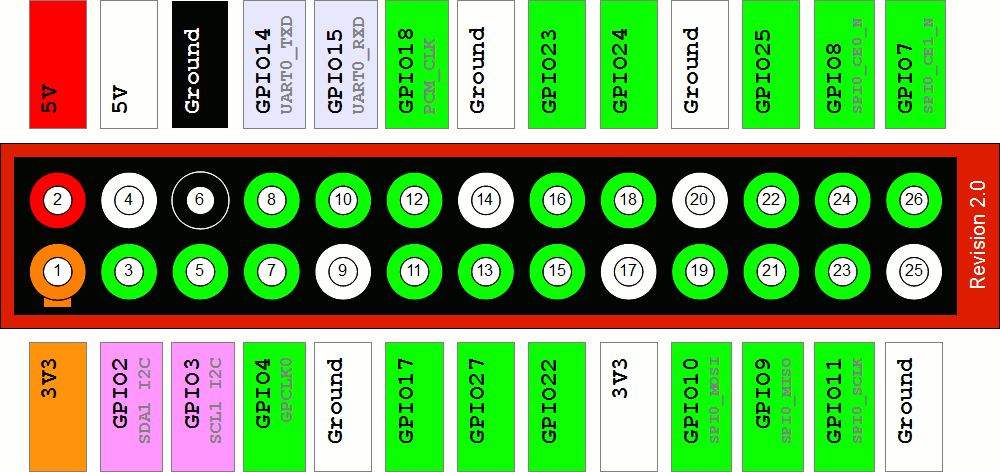
\includegraphics[width=0.45\textwidth,natwidth=610,natheight=642]{pictures/ModelAB.png}
    \caption{GPIO pins \protect\cite{gpioHeader}}
    \label{fig:ModelAB}
\end{figure}

The GPIO.BCM option means that the program is referring to the pins by the "Broadcom SOC channel" number, these are the numbers after "GPIO" in the green rectangles around the outside of the diagram above.
\newline
\newline
Unfortunately, BCM numbers changed between versions of the Model B, and is necessary to work out which one will be used. So it may be safer to use BOARD numbers if more than one pi will be used in a project.

\paragraph{Pigpio}
%http://abyz.co.uk/rpi/pigpio/python.html
Pigpio \cite{Pigpio} is a Python module for the Raspberry which talks to the pigpio daemon to allow control of the general purpose input outputs (GPIOs). Pigpio Python scripts may be run on Windows, Macs, and Linux machines. Only the pigpio daemon needs to be running on the RPi.
\newline
\newline
Pigpio provides all the standard gpio features and in addition it provides hardware timed PWM suitable for servos, LEDs, and motors and samples/timestamps gpios 0-31 up to 1 million times per second (default 200 thousand).


\section{RELATED WORK}
\label{sec:relatedWork}
As mentioned in the introduction, there is no specific library to work with python applied to Raspberry Pi, which provides a wide variety of sensors but there are some projects of such libraries for Arduino, and libraries for a particular set of sensors, which will be shown below.
\newline
\newline
%%%%%%%%%%%%%%%%%%%%%%%%%%%%%%%%%%%%%%%%%%%%%%%%%%%%%%%%%%%%%%%%%%%%%%%%%%%%%%%%%%%%%%%%%%%%%%%%%%%%%%%%
\subsection{PrivateEyePi}
PrivateEyePi\cite{Privateeyepi} is a project developed for security/automation that uses binds programming and electronics. This is an open source project that is free of charge and can be copied, shared and modified without restriction. The user can use the Raspberry Pi or an tiny wireless Arduino to connect sensors and send data over the Internet.
\newline
\newline
PrivateEyePi Provides tutorials for users explaining how to build, wire, convert the sensor to a wireless battery operated IOT device and how to connect it to the Internet. The project also provides a cloud based alarm system where the client can group sensors using zones. Zones can be activated and alarms triggered based on rules that can be defined.
\newline
\newline
Some sensors, like relay switches, can be controlled through the Internet. Users can also control the alarm system through the PrivateEyePi web based dashboard, which allows monitor status of sensors and view temperature and humidity readings in real time from the Internet. This dashboard can be seen in figure~\ref{fig:PrivateEye}.
\newline
\newline
 Historical information is provided by the analytics module. The library provides also a sophisticated rules engine that permit create rules that are processed in real time to create alerts. Those methods require parameters like sensor values, time of day, days of week, alarm activated/deactivated to define rules specific to individual sensors.     
Sensors that PrivateEyePi provides PIR motion sensor, DS18B20 digital thermometer, DHT22 for temperature and humidity readings and a generic water sensor.
%PICTURE FONT: http://projects.privateeyepi.com/
\begin{figure}[h]
\centering
    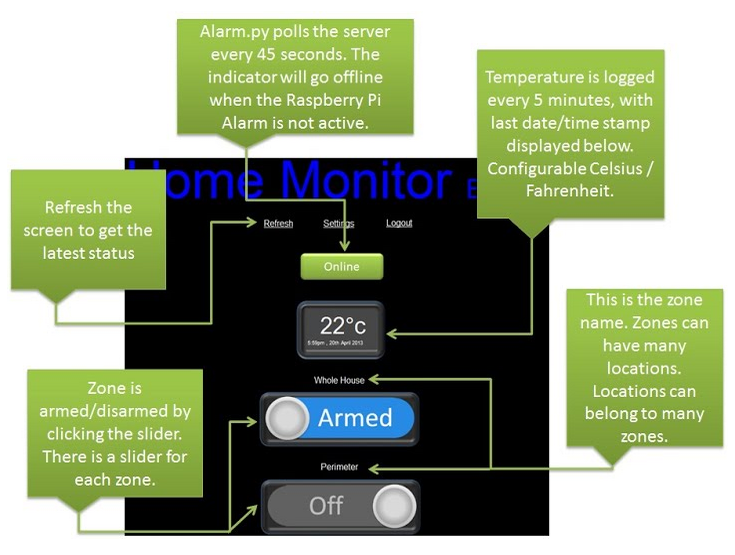
\includegraphics[width=0.5\textwidth,natwidth=610,natheight=642]{pictures/dashboardPrivateeye.png}
    \caption{PrivateEyePi web based dashboard\protect\cite{Privateeyepi}}
    \label{fig:PrivateEye}
\end{figure}

%%%%%%%%%%%%%%%%%%%%%%%%%%%%%%%%%%%%%%%%%%%%%%%%%%%%%%%%%%%%%%%%%%%%%%%%%%%%%%%%%%%%%%%%%%%%%%%%%%%%%%%%

\subsection{Pingo}
%\footnote{\url{http://www.pingo.io/docs/}} ou /cite{Pingo}
Pingo\footnote{\url{http://www.pingo.io/docs/}} is an uniform python API to program devices like the Raspberry Pi, Arduino, pcDuino, Intel Galileo etc. It's an object-oriented API where each board is an instance of a Board subclass. Every board has a dictionary called pins which lists all GPIO pins on the board. Each pin is an instance of a Pin subclass with attributes that users can inspect to learn about its capabilities.
\newline
\newline
To use pingo, the first step is to instantiate a Board. Each Pingo driver is a concrete board subclass. Two such classes are \textit{pingo.rpi.RaspberryPi} and \textit{pingo.arduino.ArduinoFirmata}. Pingo can automatically detect the board in most common cases.  \textit{pingo.detect.MyBoard()} will return an suitable board instance if the script is running on a supported board. If Pingo is running on an unsupported machine (eg. a notebook), it will try to find a connected Arduino using the Firmata protocol via USB and – if successful – will return a \textit{pingo.arduino.ArduinoFirmata} instance.
\newline
\newline
Once having a board instance, it’s possible to access its pins through the board.pins dictionary:
\renewcommand{\theFancyVerbLine}{
  \sffamily\textcolor[rgb]{0.5,0.5,0.5}{\scriptsize\arabic{FancyVerbLine}}}
\begin{minted}[mathescape,
               linenos,
               numbersep=0pt,
               gobble=0,
               frame=lines,
               framesep=2mm]{python}

  import pingo
  from time import sleep

  board = pingo.detect.MyBoard()
  led_pin = board.pins[13]
  led_pin.mode = pingo.OUT

  while True:
    led_pin.hi()
    sleep(1)
    led_pin.lo()
    sleep(1)	
\end{minted}


%%%%%%%%%%%%%%%%%%%%%%%%%%%%%%%%%%%%%%%%%%%%%%%%%%%%%%%%%%%%%%%%%%%%%%%%%%%%%%%%%%%%%%%%%%%%%%%%%%%%%%%%
%[Jefferson Jardem Izaias de Souza1 , Luís Bruno Pereira do Nascimento1 , Paulo Rodrigues dos Santos Filho2]
\subsection{PySerial}
The work from \cite{dearduino} describes a library that uses python called pySerial using serial port to communicate with Arduino mainly, but also with Python running on Windows, Linux, BSD (possibly any POSIX compliant system), Jython and IronPython (.NET and Mono). It encapsulates the access for the serial port and provides back-ends for Python. The module named "serial" automatically selects the appropriate back-end.
\newline
\newline
Features:
\begin{itemize}
\item Same class based interface on all supported platforms.
\item Access to the port settings through Python properties.
\item Support for different byte sizes, stop bits, parity and flow control with RTS/CTS(Request to Send/Clear to Send) and/or Xon/Xoff.
\item Working with or without receive timeout.
\item File like API with “read” and “write” ("readline" etc. also supported).
\item Files in this package are 100\% pure Python.
\item The port is set up for binary transmission. No NULL byte stripping, carriage return-linefeed translation(CR-LF) etc. (which are many times enabled for POSIX). This makes this module universally useful.
\item Compatible with I/O library (Python 2.6+)
\item RFC 2217 client (experimental), server provided in the examples.
\end{itemize}

That work \cite{dearduino}, describes the use of LM35 (temperature sensor) and a Light Dependent Resistor.
\newline
\newline
%%%%%%%%%%%%%%%%%%%%%%%%%%%%%%%%%%%%%%%%%%%%%%%%%%%%%%%%%%%%%%%%%%%%%%%%%%%%%%%%%%%%%%%%%%%%%%%%%%%%%%%%
%http://playground.arduino.cc/Main/DHTLib
\subsection{DHTLib}
%\footnote{\url{http://playground.arduino.cc/Main/DHTLib}} ou \cite{DHTLib}
Arduino DHTLib\footnote{\url{http://playground.arduino.cc/Main/DHTLib}} is a library for reading temperature and humidity from sensors of HDT11's family, such as DHT11, DHT21, DHT22, DHT33 e DHT44, applied to Arduino. 
\newline
\newline
The interface supports only one function for reading humidity and temperature from the sensors and store it in two members of the class. The \textit{read()} function verifies the checksum of the data transmission and it has a time out function. If there is a checksum error the values of temperature and/or humidity might still be valid.
\newline
\newline
The class has 6 read functions \textit{read11(PIN)}, \textit{read(PIN)} and \textit{readxx(PIN)} which have essentially the same interface. They read the DHT connected to PIN, and fill the two class members temperature and humidity. Multiple reads from these class members (Humidity and Temperature) will return the same (previous) values until a new read is done.
\newline
\newline
In case of a DHTLIB\_ERROR\_TIMEOUT, humidity and temperature will get the value DHTLIB\_INVALID\_VALUE. In case of DHTLIB\_ERROR\_CHECKSUM the values of humidity and temperature are left unchanged as it is impossible to determine which byte failed in the checksum. The programmer will decide what to do. One can compare with previous value, but better reread the sensor.
\newline
\newline
%%%%%%%%%%%%%%%%%%%%%%%%%%%%%%%%%%%%%%%%%%%%%%%%%%%%%%%%%%%%%%%%%%%%%%%%%%%%%%%%%%%%%%%%%%%%%%%%%%%%%%%%
%https://code.google.com/p/arduino-new-ping/
\subsection{NewPing}
NewPing Library for Arduino\footnote{\url{https://code.google.com/p/arduino-new-ping/}}  is an ultrasonic sensor library for Arduino that was developed to work with sensors SR04, SRF05, SRF06, DYP-ME007 and Parallax PING)))\textsuperscript{TM}. Intended to use with Sketches (Software written using Arduino), the library is written with C++.
\newline
\newline
Features:
\begin{itemize}
\item Works with many different ultrasonic sensor models: SRF05, SRF06, DYP-ME007, Parallax PING)))\textsuperscript{TM} and SR04.
\item Option to interface with all but the SRF06 sensor using only one Arduino pin.
\item Doesn't lag for a full second if no ping echo is received like all other ultrasonic libraries.
\item Ping sensors consistently and reliably at up to 30 times per second.
\item Timer interrupt method for event-driven sketches.
\item Built-in digital filter method \textit{ping\_median()} for easy error correction.
\item Uses port registers when accessing pins for faster execution and smaller code size.
\item Allows setting of a maximum distance where pings beyond that distance are read as no ping "clear".
\item Ease of using multiple sensors (example sketch that pings 15 sensors).
\item More accurate distance calculation (cm, inches and microseconds).
\item Doesn't use pulseIn, which is slow and gives incorrect results with some ultrasonic sensor models.
\item Actively developed with features being added and bugs/ issues addressed. 
\end{itemize}

%%%%%%%%%%%%%%%%%%%%%%%%%%%%%%%%%%%%%%%%%%%%%%%%%%%%%%%%%%%%%%%%%%%%%%%%%%%%%%%%%%%%%%%%%%%%%%%%%%%%%%%%
%https://github.com/adafruit/Adafruit-Raspberry-Pi-Python-Code
\subsection{Adafruit Raspberry Pi Python Code}
Adafruit's Raspberry-Pi Python Code Library\footnote{\url{https://github.com/adafruit/Adafruit-Raspberry-Pi-Python-Code}} is the most closed work with this paper. Written by Limor Fried, Kevin Townsend and Mikey Sklar under BSD license for controlling a variety of Adafruit electronics with a Raspberry Pi, a growing collection of libraries and example python scripts are provided.
\newline
\newline
This library provides a collection of python scripts to work with sensors, providing classes that can be used to measure values from the sensor that the class implements. 
\newline
\newline
Despite being a library with a considerable amount of sensors, if the user wants to change the type of sensor in a project, is necessary review the documentation of the new sensor to be used because the library does not use a standard for equivalent sensors.

\subsection{Discussions and Observations}
\label{sec:justification}
As with other platforms, Raspberry Pi allows coupling several sensors whose handling can be made from raspberry-gpio-python or any other API available. On other platforms, such as Arduino, the APIs provide libraries that encapsulate the complexity of implementation and offer only the interface to use. These libraries do not yet exist formally for those who want to use Python as a development language for Raspberry Pi.
\newline
\newline
This may be a consequence of run under the Linux kernel which is not suitable for real time applications, a multitasking O/S and another process may be given priority over the CPU, causing jitter in the program \cite{Oracle}.
\newline
\newline
The library proposed reconciles the use of an integrated circuit platform with microcontroller , thereby strengthening the use of free hardware, aiming to solve problems of a physical nature, with several components used to the extent that platform, allowing it to have a greater range of utility, potentiating their functions. Among the components which have greater relevance are the sensors that capture and process variations in the environment into electrical signals that are identified by the circuit platform. With the use of a high-level programming language make the communication interface between the computer and the microcontroller, capturing data sent to the computer, allowing the user to make the necessary analysis.


\section{LIBSENSORPY}
\label{sec:proposedModel}
Many small embedded systems exist to collect data from sensors, analyses the data, and either take an appropriate action or send that sensor data to another system for processing. One of the many challenges of embedded systems design is the fact that parts that are used today may be out of production tomorrow, or system requirements may change and may will be needed to choose a different sensor down the road.
\newline
\newline
Creating new drivers is a relatively easy task, but integrating them into existing systems is both error prone and time consuming since sensors rarely use the exact same units of measurement. By reducing all data to a single sensors/event family type and settling on specific, standardized SI units for each sensor family the same sensor types return values that are comparable with any other similar sensor. This enables users to switch sensor models with very little impact on the rest of the system, which can help mitigate some of the risks and problems of sensor availability and code reuse.
\newline
\newline
LibsensorPy is an extensible library, which allows the user to interact with environment through sensors and actuators coupled to the Raspberry Pi as well as add new sensors / actuators and easy way to practice. Often programmers, who have no knowledge in electronics, and engineers who do not have programming experience need to create ubiquitous systems, requiring a lot of work to implement system's abstractions, configure logic connections between sensors and the microcontroller, capture, understand and process the data in order to make them readable.
\newline
\newline 
With the proposed system, the user only need to worry about using the data that the solution delivery already processed since the system provides the abstractions of the main necessary resources for the processing and, if desired, inform the library in which pins the sensors are connected, if the user does not want to use default configuration of each sensor. Conversions between units of measure are also provided, facilitating and universalizing the use of the library.
\newline
\newline 
LibsensorPy provides a simple abstraction layer between user's application and the actual sensor Hardware, allowing to drop in any comparable sensor with only one or two lines of code to change in the project that uses the library. This change is essentially in the constructor since the functions to read data and get information about the sensor are defined in the family sensor class, e.g. UltrasonicSensor class.
\newline
\newline
This is important useful for two reasons:

\begin{enumerate}
\item Users can use the data right away because it's already converted to SI units that is understandable and can compare, rather than meaningless values like 0..1023.
\item Because SI units are standardized in the sensor library, users can also do quick sanity checks working with new sensors, or drop in any comparable sensor if needed better sensitivity or if a lower cost unit becomes available, etc.
\end{enumerate}

Light sensors will always report units in lux, pressure sensors will always report units in hPa and so forth, freeing user up to focus on the data, rather than digging through the datasheet to understand what the sensor's raw numbers really mean. Also the library offer methods to convert the standard SI to other measurement unit, thus who are using the library can abstracts these conversions. A sheet of Standardized SI values and measurable units and conversions for each sensor can be seen in appendix~\ref{sec:Units}.
\newline
\newline
The purpose of this work is the focus on library's usability and the abstraction from the way that this library interacts with sensors/actuators to capture data, besides contributing to the open source community and the growing community of developers for the Raspberry Pi.
\newline
\newline
The technologies used to develop the tool were basically the Python language and RPI.GPIO and PigPio modules that provide connection abstractions to basic pins and the special pins I2C, UART, SPI and PWM.
\newline
\newline
To develop this project was adopted the object-oriented analysis and design (OOAD). OOAD is a popular technical approach to analyzing, designing an application, system, or business by applying the object-oriented (OO) paradigm and visual modeling throughout development life cycles to foster better stakeholder communication and product quality.
\newline
\newline
According to the popular guide Unified Process, OOAD in modern software engineering is best conducted in an iterative and incremental way. Iteration by iteration, the outputs of OOAD activities, analysis models for Object-oriented analysis (OOA) and design models for Object- oriented design (OOD) respectively, were refined and evolved continuously driven by key factors like usability and efficiency.
\newline
\newline
Object-oriented approach is ambitious: it encompasses the entire software lifecycle. When examining object-oriented solutions, should be checked that the method and language, as well as the supporting tools, apply to analysis and design as well as implementation and maintenance. The language, in particular, should be a vehicle for thought which will help through all stages of the work. In this context, Python was essentially fundamental since it provides fully object oriented functionalities that attend the project's requirements. 
\newline
\newline
Using Object-oriented modeling, the work is divided in two aspects: Modeling dynamic behaviors like events and use cases, and the modeling of static structures like classes and components. OOA and OOD were two distinct abstract levels (i.e. the analysis level and the design level) during OOM. The Unified Modeling Language (UML), a popular international standard languages used for object-oriented modeling was used. The benefits of OOM are:

%\subsubsection{Efficient and effective communication}
\begin{itemize}
\item Efficient and effective communication:
\end{itemize}

Users typically have difficulties in understanding comprehensive documents and programming language codes well. Visual model diagrams can be more understandable and can allow users and stakeholders to give developers feedback on the appropriate requirements and structure of the system. A key goal of the object-oriented approach is to decrease the "semantic gap" between the system and the real world, and to have the system be constructed using terminology that is almost the same as the stakeholders use in everyday business. Object-oriented modeling is an essential tool to facilitate this.
\newline
\newline
\begin{itemize}
\item Useful and stable abstraction:
\end{itemize}
%\subsubsection{Useful and stable abstraction}

Modeling helps coding. A goal of most modern software methodologies is to first address "what" questions and then address "how" questions, i.e. first determine the functionality the system is to provide without consideration of implementation constraints, and then consider how to make specific solutions to these abstract requirements, and refine them into detailed designs and codes by constraints such as technology and budget. Object-oriented modeling enables this by producing abstract and accessible descriptions of both system requirements and designs, i.e. models that define their essential structures and behaviors like processes and objects, which are important and valuable development assets with higher abstraction levels above concrete and complex source code.
\newline
\newline
Patterns used:
\begin{itemize}
\item Abstract Factory;
\item Singleton;
\item Observer;
\item Composite;
\end{itemize}

%\subsection{Functional Requirements}
In the table \ref{table:rf} are defined the main functional requirements in order to be able to meet all the objectives proposed by libsensorPy library. Are characterized as non-functional requirements for the proper functioning of libsensorPy the items in table \ref{table:rnf}.
%\subsection{Non-functional Requirements} 
 
\begin{table}[h]
 \caption{Functional requirements of libsensorPy}
 \label{table:rf}
 \begin{tabular}{|l|p{5.5cm}|l|}
 \hline  
 Id & Functional Requirements & Actor \\
 \hline  
 RF01 & Collect data sent by the sensors via the GPIO pins; & Library \\
 \hline 
 RF02 & Manipulate data sent by the sensors, turning them into readable data to the user; & User \\
 \hline 
 RF03 & Allow the user to set the pins to be used for connection between sensor and Raspberry; & User \\
 \hline 
 RF04 & Allow the creation of composite sensors, enabling a single sensor to measure more than one physical greatness; & User \\
 \hline 
 RF05 & Allow configuration of a set of conditions (events) that, When met, trigger an action. & User \\
\hline  
\end{tabular}
\end{table}



\begin{table}[h]
 \caption{Non-functional requirements of libsensorPy}
 \label{table:rnf}
 \begin{tabular}{|l|p{4.7cm}|l|}
 \hline  
 Id & Non-Functional Requirements & Category \\
 \hline  
 RNF01 & The library must allow addition of new sensors/families; & Extensibility\\
 \hline  
 RNF02 & The data reported by the application must be faithful to that presented in the environment; & Confidence \\
 \hline 
 RNF03 & The library should be usable in any Raspberry Pi model ; & Portability \\
 \hline 
 RNF04 & The library will be developed using Python language; & Software \\
\hline  
\end{tabular}
\end{table}

%\subsection{Why not to use Java}
%At the beginning of this project was decided to develop the library using Java as the programming language, since these libraries do not yet exist formally for those who want to use Java as a development language. It could be a consequence of the recent adoption of the use of Java for Raspberry (when compared with other APIs and platforms). But after implement the first sensors, the DHT11 and HC-SR04, when tried to test, no data were provided from the sensors.
%\newline
%\newline
%After some research about what could be the problem, was found that is not possible to assume that invoking sleep will suspend the thread for precisely the time period specified, since \textit{Thread.sleep()} and the \textit{Thread.Join()} methods are dependent on the operating system and the version of the JVM \cite{Oracle}.
%%fonte: http://docs.oracle.com/javase/tutorial/essential/concurrency/sleep.html
%\newline
%\newline
%These sensors need to wait microseconds between send a signal to the sensor and get back the data read from it, And because of this not real time property from both Java and the Raspberry Pi, the library couldn't read data from those sensors. After that the project was moved on to change the programming language and was decided to use python, especially because it's the recommended programming language by the Raspberry Pi developers.

\subsection{Architecture of LibsensorPy}
The system consists of a module that implements the abstract factory pattern, guaranteeing independence of how products are created, composed and represented. For that, the system must be configured with one of multiple product families (family of sensors). It provides one product class library: sensors, actuators and events related to the family of each sensor, but are only revealed their interfaces, not their implementations. Figure~\ref{fig:classDiagram} shows the main class diagram.
\begin{figure*}[ht]
\centering
    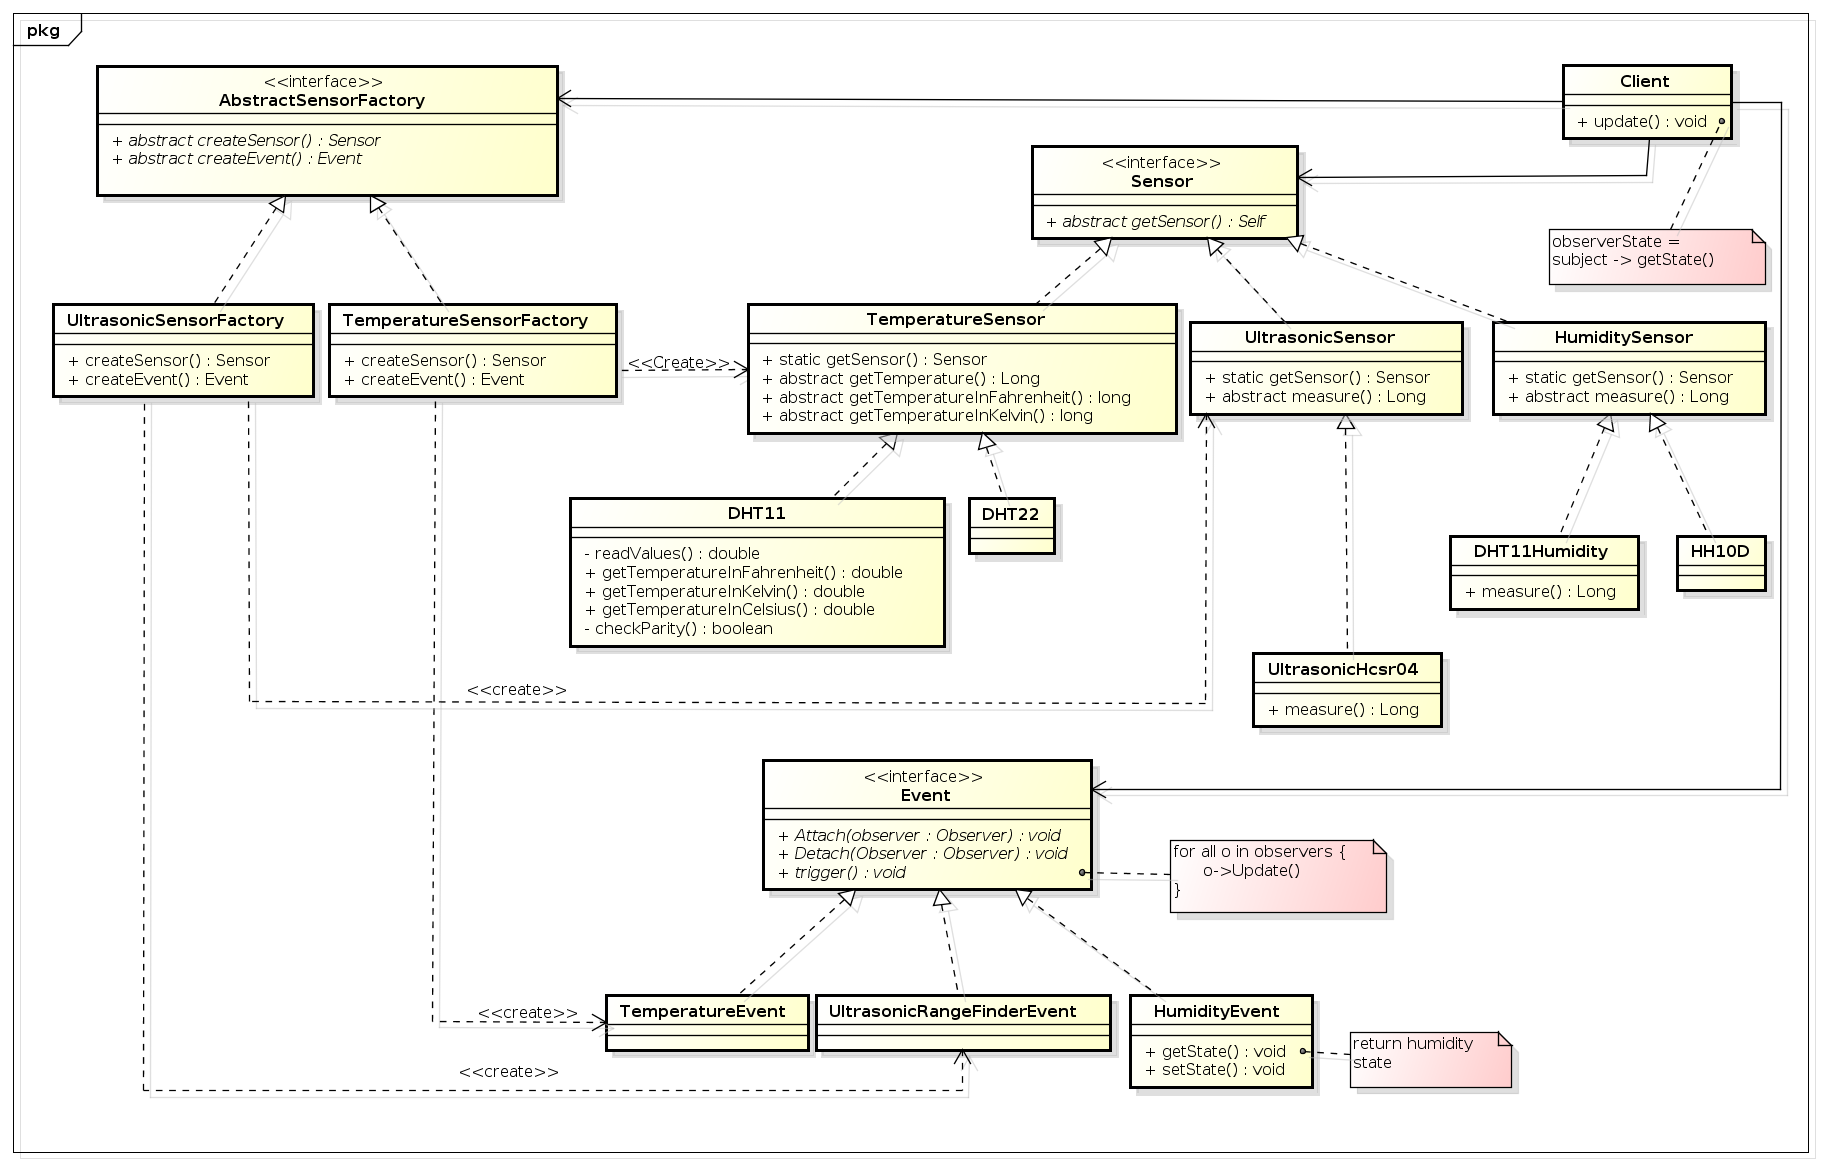
\includegraphics[resolution=300,width=1.0\textwidth,natwidth=610,natheight=642]{pictures/ClassDiagram2.png}
    \caption{Class diagram}
    \label{fig:classDiagram}
\end{figure*}
\newline
\newline
Main components:
\begin{itemize}
\item AbstractSensorFactory: Declares an interface for operations that create abstract sensors and events;
\item ConcreteFactories: Implement operations to create concrete sensors and events;
\item AbstractSensor: Declares an interface for sensors;
\item AbstractActuator: Declares an interface to the actuators;
\item AbstractEvent: declares an interface for the events;
\item ConcreteSensors, ConcreteActuators, ConcreteEvents: Define the concrete objects to be created by the corresponding concrete factory and implement AbstractSensor, AbstractActuator and AbstractEvent interfaces respectively.

\end{itemize}

A single instance of the concrete factory is created at run-time, using the Singleton pattern. This factory creates products with a particular implementation. To create other products from a different family, one should use a different factory. The concrete factory class being used appears only once in the application, facilitating changes. The product family changes all at once, promoting consistency across products, ensuring that used objects are all of the same family, represented by the concrete factory being used.
\newline
\newline
Due to some sensors belong to more than one family (measure more than one physical quantity), the library allows the use of composite-type sensors composed of basic sensors. This ability is facilitated by Python feature that allow multiple inheritance. For example, the DHT11 sensor is capable of measuring temperature and humidity so, were then created three sensors: Two basic sensor from distinct families (DHT11Temperature to measure temperature and DHT11Humidity to the family of humidity sensors) and a composite sensor (DHT11Composite) that aggregates the two basic sensors. The idea of the separation of basic and composite sensors is to allow the creation of lighter objects, if the user just want a sensor that measures only a physical quantity. The composite pattern structure allows basic and composite sensors being viewed by the user in the same way. This structure can see in figure~\ref{fig:composite}.
\newline
\begin{figure*}[ht]
\centering
    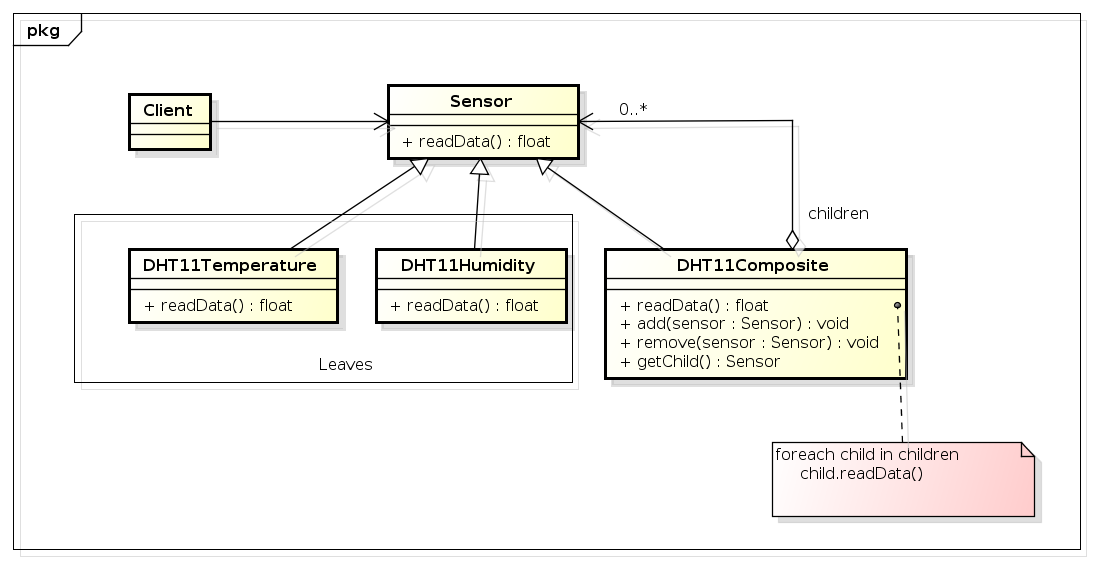
\includegraphics[width=1.0\textwidth,natwidth=610,natheight=642]{pictures/composite.png}
    \caption{Composite class diagram}
    \label{fig:composite}
\end{figure*}


The interactions between the user and the library are described in the use case diagram  in figure~\ref{fig:useCase}. The sequence diagram for the creation and capture of data by the sensor can be seen in figure~\ref{fig:sequence}.
\begin{figure*}[ht]
\centering
    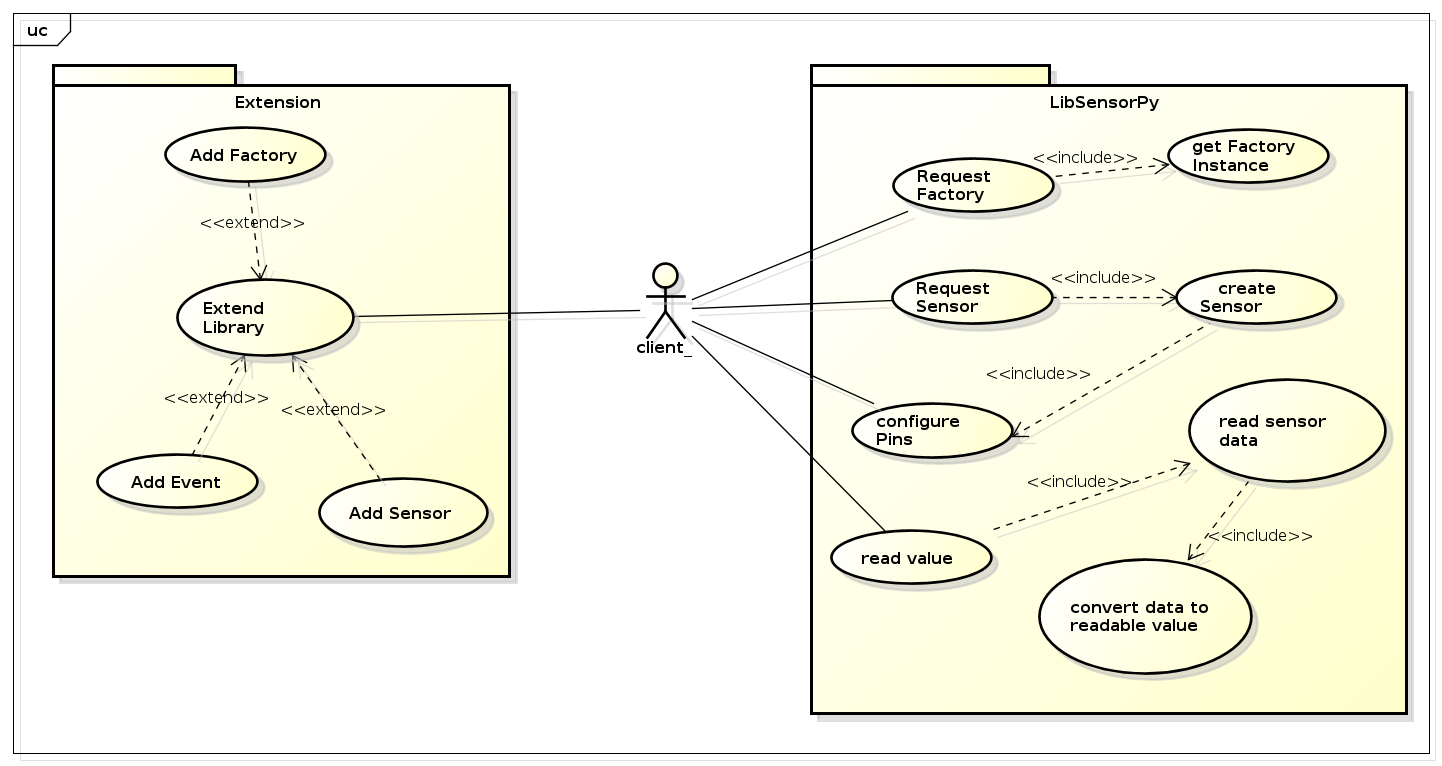
\includegraphics[width=1.0\textwidth,natwidth=610,natheight=642]{pictures/UseCaseDiagram.png}
    \caption{Use Case diagram}
    \label{fig:useCase}
\end{figure*}

\begin{figure*}[t]
\centering
    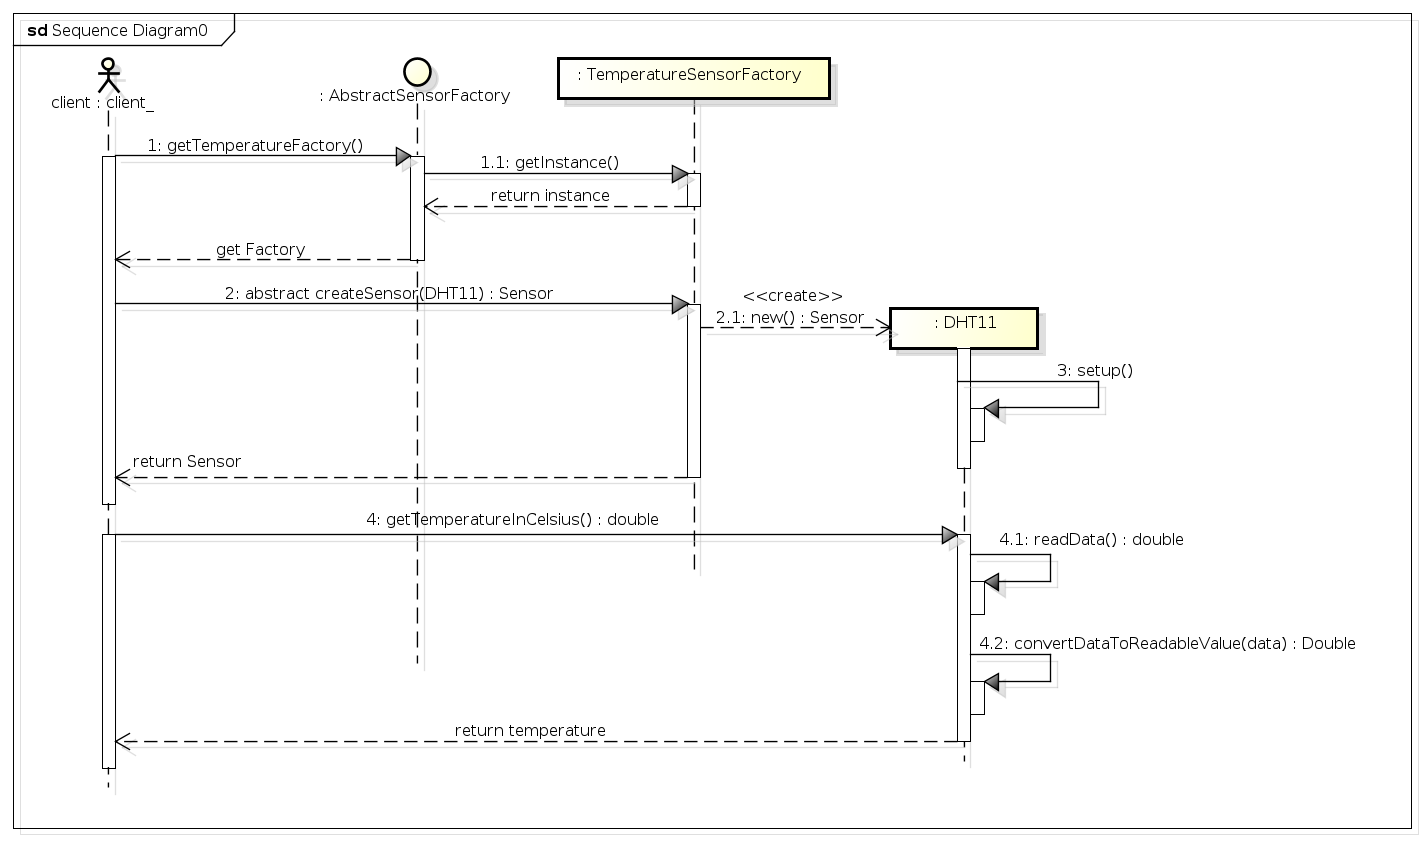
\includegraphics[resolution=300,width=1.0\textwidth,natwidth=610,natheight=642]{pictures/SequenceDiagram3.png}
    \caption{Sequence diagram}
    \label{fig:sequence}
\end{figure*}

\subsubsection{Architectural Style}
The libsensorPy presents characteristics of three architectural styles: 
\begin{itemize}
\item Traditional, influenced by programming language: OO;
\item Based on Implicit Invocation: Event Based; 
\item Layered Style: Virtual Machine.
\end{itemize}

The traditional style adopted reflects the basic relationships of organization and control flow between components provided by Python language. The only provided structure is a set of objects whose lifetime varies according to its uses. This library uses connectors type procedure call and event. Procedure call connectors model the control flow by invocation techniques and perform data transfer between components involved through the use of parameters. Examples of procedure call connectors include functions, procedures,  object oriented methods, callback and system calls.
\newline
\newline
The Virtual Machine style is applied between the hardware and the libsensorPy library, using procedure calls as connectors between the layers. The system has thus the layers:
\begin{itemize}
\item Physical: GPIO
\item Operating System
\item RPi.GPIO
\item LibsensorPy
\end{itemize}

\begin{figure}[h]
\centering
    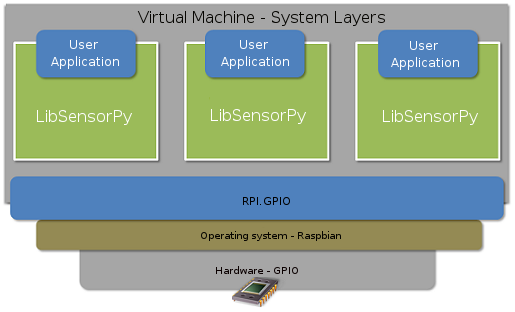
\includegraphics[width=0.4\textwidth,natwidth=610,natheight=642]{pictures/machinelayers.png}
    \caption{LibsensorPy's layers}
    \label{fig:layers}
\end{figure}

The event-based style is an architectural style based on implicit invocation that provides an indirect interaction between loosely coupled components facilitating the adaptation and improving system scalability. The components of the Event type (TemperatureEvent, SmokeEvent, etc.) communicate only via events transmitted by an event connector. This connector then relays the events for all components of the Observer type showing interest in the event in question (Observer pattern), thereby improving the efficiency of distribution of events.

\subsubsection{Architectural Pattern}
This project was developed under the architectural pattern Sense-Compute-Control (SCC). This pattern is typically used in the structuring of embedded control applications. Second \cite{taylor2009software}, a Sense/Compute/Control (SCC) application is one that interacts with the physical environment. Such applications are pervasive in domains such as building automation, assisted living, and autonomic computing. SCC applications can be defined according to an architectural pattern involving four kinds of components, organized into layers \cite{edwards2009architecture}: 
\begin{enumerate}
\item Sensors at the bottom, which obtain information about the environment; 
\item Then context operators, which process this information; 
\item Then control operators, which use this refined information to control;
\item Actuators at the top, which finally impact the environment
\end{enumerate}

%PICTURE FONT: http://pt.slideshare.net/DamienCassou/architecturedriven-programming-for-sensecomputecontrol-applications
\begin{figure}[h]
\centering
    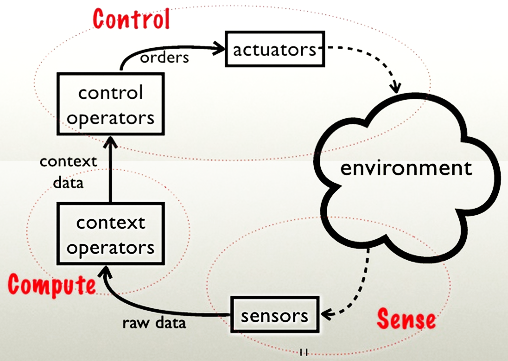
\includegraphics[width=0.45\textwidth,natwidth=610,natheight=642]{pictures/senseComputeControl2.png}
    \caption{Sense-Compute-Control environment \protect\cite{DamienCassou}.}
    \label{fig:scc}
\end{figure}

Each layer corresponds to a separate class of components: 
\begin{itemize}
\item Sensors send information sensed from the environment to the context operator layer through data sources. Sensors can both push data to context operators and respond to context operator requests. The term "sensor" is used both for entities that actively retrieve information from the environment, such as system probes, and entities that store information previously collected from the environment, such as databases.
\item Context operators refine (aggregate and interpret) the information given by the sensors. Context operators can push data to other context operators and to control operators. Context operators can also respond to requests from parent context operators. 
\item Control operators transform information given by the context operators into orders for the actuators. 
\item Actuators trigger actions on the environment.
\end{itemize}

Sensors are proactive or reactive components whereas context operators, control operators and actuators are always reactive. These properties ensure that SCC applications are reactive to the environment state. That is, all computation is initiated by an observer interaction with a sensor.
\newline
\newline
As the underlying architecture is component-based, the application can be fully distributed. To prevent concurrent handling of events in a component, all interactions of a component are queued and executed one at a time, sequentially.
\newline
\newline
The application follows the five basic principles of design oriented to objects, called "SOLID" \cite{DanielPace}. Addressed initially by Robert Martin, in an article called Principles Of Ood, the author elaborates five-oriented programming techniques to objects where each technique is one of SOLID letters of the word. These five principles are:
\begin{itemize}
\item Single Responsibility Principle;
\item Open Closed Principle;
\item Liskov Substitution Principle;
\item Interface Segregation Principle;
\item Dependency Inversion Principle;
\end{itemize} 

Figure~\ref{fig:view} shows the library's structural view.
\begin{figure*}[ht]
\centering
    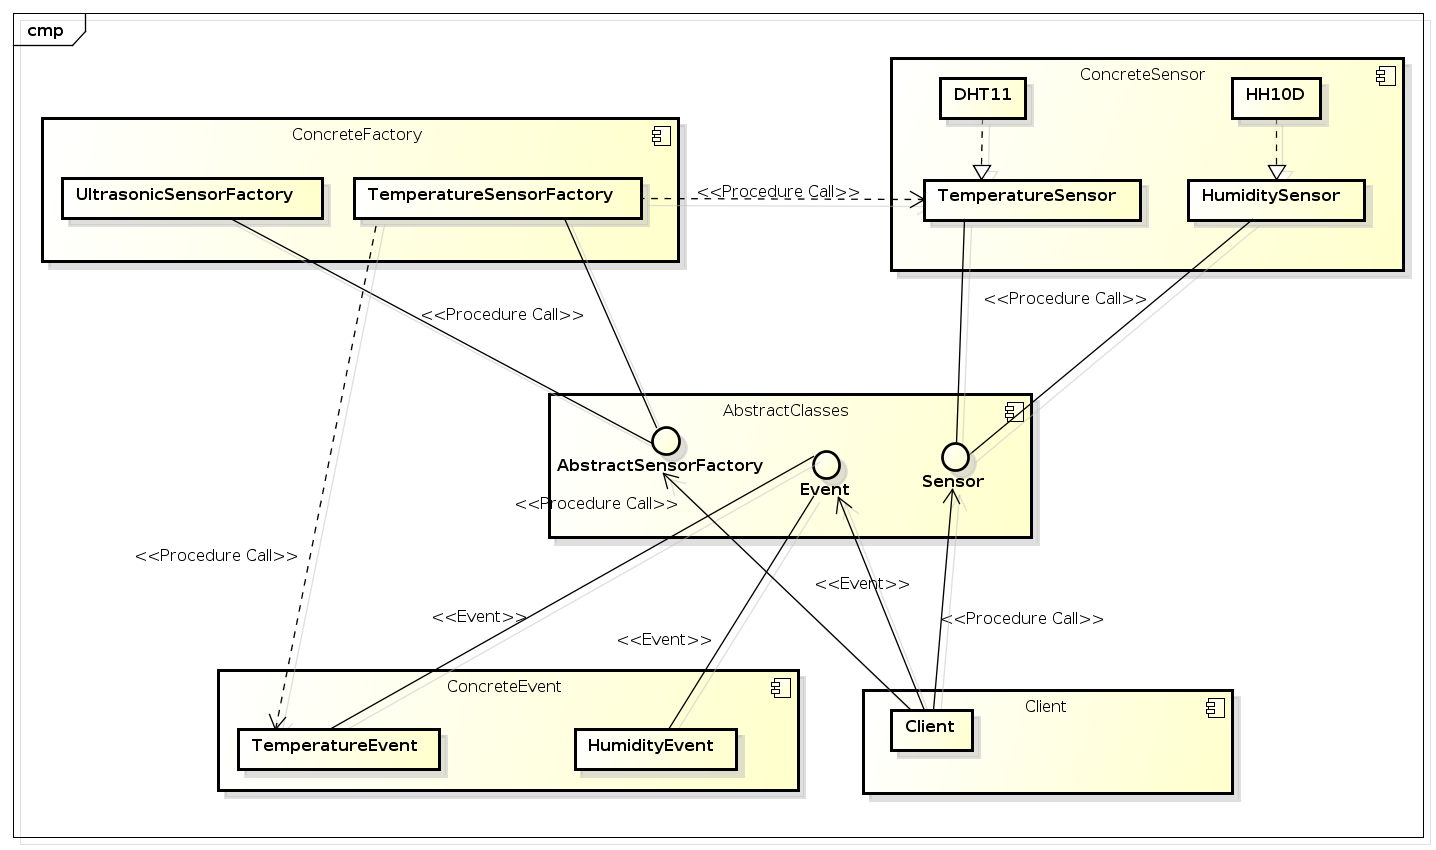
\includegraphics[width=1.0\textwidth,natwidth=610,natheight=642]{pictures/VisaoEstrutural.png}
    \caption{LibsensorPy's structural view}
    \label{fig:view}
\end{figure*}

\subsection{What is needed to install LibsensorPy?}
Before use LibsensorPy is necessary to configure and enable SPI and I2C ports on raspperry:
\renewcommand{\theFancyVerbLine}{
  \sffamily\textcolor[rgb]{0.5,0.5,0.5}{\scriptsize\arabic{FancyVerbLine}}}
\begin{minted}[mathescape,
               linenos,
               numbersep=0pt,
               gobble=0,
               frame=lines,
               framesep=2mm]{bash}

  sudo apt-get install python-smbus
  sudo apt-get install i2c-tools	

\end{minted}

Check \textit{/etc/modprobe.d/raspi-blacklist.conf} if using Raspbian, and comment "blacklist i2c-bcm2708" and "blacklist spi-bcm2708" by running:

\renewcommand{\theFancyVerbLine}{
  \sffamily\textcolor[rgb]{0.5,0.5,0.5}{\scriptsize\arabic{FancyVerbLine}}}
\begin{minted}[mathescape,
               linenos,
               numbersep=0pt,
               gobble=0,
               frame=lines,
               framesep=2mm]{bash}

  sudo nano /etc/modprobe.d/raspi-blacklist.conf	

\end{minted}

And adding a \# (if its not there), on these informations: "blacklist i2c-bcm2708" and "blacklist spi-bcm2708".
\newline
\newline
For Wheezy or something-other-than-Occidentals, add the following lines to \textit{/etc/modules}: 
\renewcommand{\theFancyVerbLine}{
  \sffamily\textcolor[rgb]{0.5,0.5,0.5}{\scriptsize\arabic{FancyVerbLine}}}
\begin{minted}[mathescape,
               linenos,
               numbersep=0pt,
               gobble=0,
               frame=lines,
               framesep=2mm]{bash}

  i2c-dev
  i2c-bcm2708
  spi-bcm2708	

\end{minted}

Install pigpio:
\begin{minted}[mathescape,
               linenos,
               numbersep=0pt,
               gobble=0,
               frame=lines,
               framesep=2mm]{bash}

  wget abyz.co.uk/rpi/pigpio/pigpio.zip
  unzip pigpio.zip
  cd PIGPIO
  sudo make
  sudo make install	
\end{minted}

install pip:
\begin{minted}[mathescape,
               linenos,
               numbersep=0pt,
               gobble=0,
               frame=lines,
               framesep=2mm]{bash}

  sudo apt-get install python-pip
\end{minted}

and finally install LibsensorPy:
\begin{minted}[mathescape,
               linenos,
               numbersep=0pt,
               gobble=0,
               frame=lines,
               framesep=2mm]{bash}

  sudo pip install LibsensorPy
\end{minted}


\subsection{How to extend the library}
The Abstract Factory pattern, how it was implemented in this solution, allows the extension of the library easily, following the  open/closed principle, becoming it easy to modify and avoiding the user application does not suffer from the impact of these changes. This requires user programming skills. The user can add new sensors, events and new factories. To add new sensors, simply, besides implement the sensor class, create a concrete factory that inherits from the factory referring to the sensor family to be added and overwrite the \textit{createSensor()} method, making this method to create the new sensor, if desired, or call the create method of the superclass sensor, ensuring system compatibility.
\newline
\newline
To add a new sensor family just create a new factory that implements the abstract methods of AbstractSensorFactory interface. If desired, is possible also to create an abstract family class for this , if there is not in the library, creating thus a "contract", where attributes are specified, methods and functions that the concrete sensors classes of this family are required to implement .
\newline
\newline
Follows an example of how to extend the library: The HCSR04 class was implemented to create objects of the ultrasonic sensor HC-SR04. Being the family of ultrasonic sensors, this class was created as a subclass of UltrasonicSensor abstract class, which has the abstract methods \textit{distance\_in\_cm()} and \textit{setup()}  to be implemented. It has also created a concrete factory ExtendedUltrasonicSensorFactory, which inherits the UltrasonicSensorFactory class and overrides the \textit{createSensor()} method, as seen following:

%%%%%%%%%%%%%%%%%%%%%%%%%%%%%%%%%%%%%%%%%%%%%%%%%%%%%%%
\renewcommand{\theFancyVerbLine}{
  \sffamily\textcolor[rgb]{0.5,0.5,0.5}{\scriptsize\arabic{FancyVerbLine}}}
\begin{minted}[mathescape,
               linenos,
               numbersep=0pt,
               gobble=0,
               frame=lines,
               framesep=2mm]{python}

  '''
  Created on 29/03/2015
  @author: Junior Mascarenhas
  File: hcsr04.py
  '''
  import RPi.GPIO as GPIO
  import time
  from abstractclass.ultrasonicSensor import \
  		UltrasonicSensor

  class HCSR04(UltrasonicSensor):
      '''
      classdocs
      '''

      def __init__(self, trigger = 18, echo = 27):
          '''
          Constructor
          '''
          UltrasonicSensor.__init__(self)
          self.__distance = ""
          self.__trigger = trigger
          self.__echo = echo
          self.setup()
        
      def setup(self):
          GPIO.setmode(GPIO.BCM)
          GPIO.setwarnings(False)

      def changeSetup(self, trigger, echo):
          self.__trigger = trigger
          self.__echo = echo

      def distance_in_cm(self):

          GPIO.setup(self.__trigger,GPIO.OUT)
          GPIO.setup(self.__echo,GPIO.IN)
          GPIO.output(self.__trigger, GPIO.LOW)
          time.sleep(0.3)
          GPIO.output(self.__trigger, True)
          time.sleep(0.00001)
          GPIO.output(self.__trigger, False)

          while (GPIO.input(self.__echo) == 0):
              signaloff = time.time()

          while GPIO.input(self.__echo) == 1:
              signalon = time.time()

          timepassed = signalon - signaloff
          self.__distance = timepassed * 17000
          return self.__distance

\end{minted}
%%%%%%%%%%%%%%%%%%%%%%%%%%%%%%%%%%%%%%%%%%%%%%%%%%%%%%%
\begin{figure*}[ht]
    \centering
    	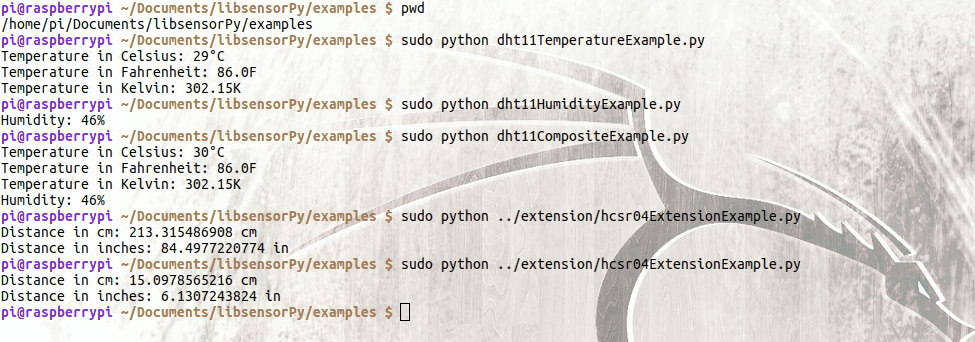
\includegraphics[width=0.9\textwidth]{pictures/tests2.png}
    		\caption{Testing the sensors}  
    		\label{fig:results}  	
\end{figure*}
%%%%%%%%%%%%%%%%%%%%%%%%%%%%%%%%%%%%%%%%%%%%%%%%%%%%%%%
\renewcommand{\theFancyVerbLine}{
  \sffamily\textcolor[rgb]{0.5,0.5,0.5}{\scriptsize\arabic{FancyVerbLine}}}
\begin{minted}[mathescape,
               linenos,
               numbersep=0pt,
               gobble=0,
               frame=lines,
               framesep=2mm]{python}

  '''
  Created on 29/03/2015
  @author: Junior Mascarenhas
  File: extendedUltrasonicSensorFactory.py
  '''

  from abstractclass.abstractSensorFactory \
      import AbstractSensorFactory
  from concretefactory.ultrasonicSensorFactory \
      import UltrasonicSensorFactory
  from hcsr04 import HCSR04

  class ExtendedUltrasonicSensorFactory\
              (UltrasonicSensorFactory):
      '''
      classdocs
      '''

      def __init__(self):
          '''
          Constructor
          '''
      @staticmethod
      def createSensor(sensorType):
          if (sensorType == "HCSR04"):
                  return HCSR04()
          else:
                  return super(sensorType)
\end{minted}

\subsection{Case Study}
\begin{figure*}[t]
    \centering
    	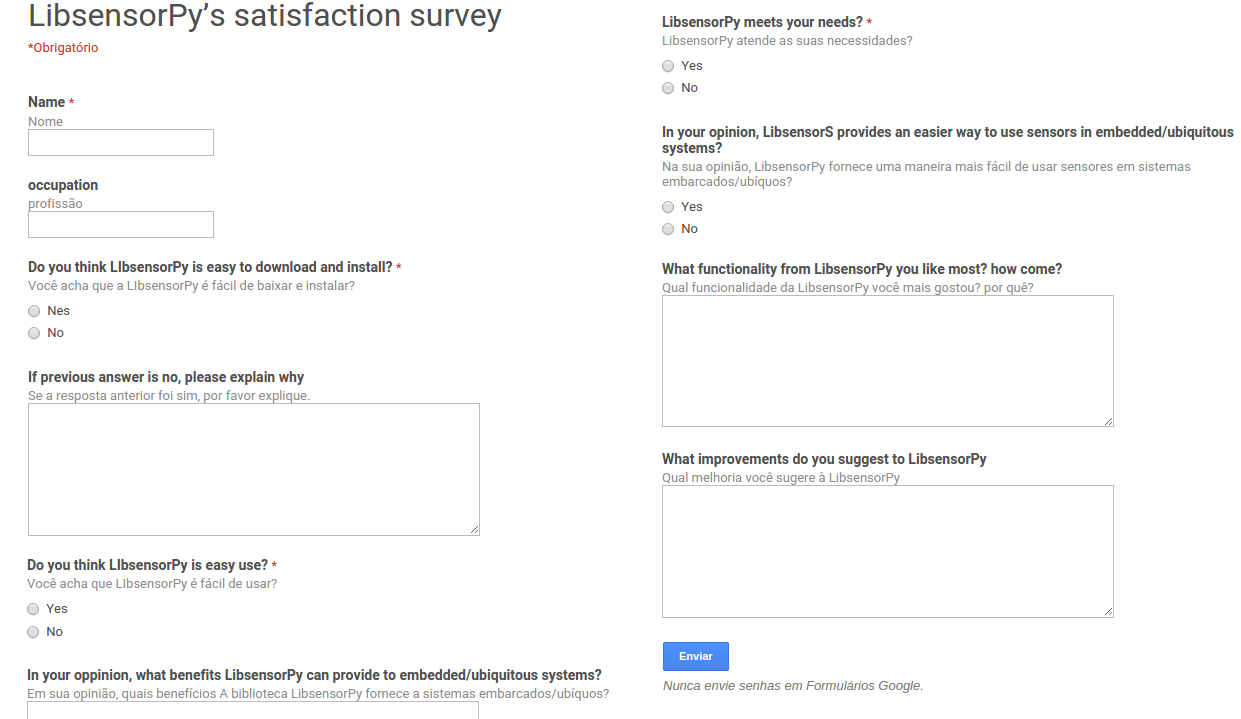
\includegraphics[width=1.0\textwidth]{pictures/survey2.png}
    		\caption{LibsensorPy's satisfaction survey}  
    		\label{fig:survey}  	
\end{figure*}
In this work the case study began with software verification tests which consisted of functional tests of LibsensorPy. These tests were performed as the system was being implemented.
\newline
\newline
Verification tests are related to the system specification, the purpose of these tests is to verify the compliance with the library's functional requirements. Tests were performed based on test cases.
\newline
\newline
Below is presented \textit{dht11CompositeExample.py}, an example of how to use the library and these example classes were used to test the library.

\renewcommand{\theFancyVerbLine}{
  \sffamily\textcolor[rgb]{0.5,0.5,0.5}{\scriptsize\arabic{FancyVerbLine}}}
\begin{minted}[mathescape,
               linenos,
               numbersep=0pt,
               gobble=0,
               frame=lines,
               framesep=2mm]{python}

  '''
  Created on 29/03/2015
  @author: Junior Mascarenhas
  File: dht11CompositeExample.py
  '''
  
  from concretefactory.compositeSensorFactory \
  	import CompositeSensorFactory

  if __name__ == '__main__':

    dht11 = CompositeSensorFactory.createSensor\
    	    ("DHT11Composite")
    print ("Temperature in Celsius: " \
    + dht11.getTemperature() + u"\u00b0" + "C")
    print ("Temperature in Fahrenheit: " \
    + dht11.getTemperatureInFahrenheit() +"F")
    print ("Temperature in Kelvin: " \
    + dht11.getTemperatureInKelvin() +"K")
    print ("Humidity: " + dht11.getHumidity() + "%")
\end{minted}
Was then given to continue the study validation tests. These tests were performed after development's completion of LibsensorPy, and was based on the library's availability to the people who are involved in ubiquitous systems development activities.
\newline
\newline
This library was presented to a post graduation student in distributed and ubiquitous computing that are developing work in this area. The main objective was to determine whether LibsensorPy meets the user needs.
\newline
\newline
At the end of the presentation this student were invited to complete the satisfaction of LibsensorPy's survey. Figure~\ref{fig:survey} shows satisfaction survey screen using Google Forms.
\newline
\newline

%\subsection{Case Study results}

The result of the case study was satisfactory. Tested sensors worked as expected, and the data reported were consistent with environment. The interviewed, during the case study, confirmed that LibsensorPy meets the user needs. However, this students made some notifications about show more use examples.
\newline
\newline
%%%%%%%%%%%%%%%%%%%%%%       MAIS CONTEUDO AQUIIIIIIIIIIIIIII %%%%%%%%%%%%%%%%%%%%%% 
The sensors HCSR04, DHT11Temperature, DHT11Humidity and DHT11Composite were tested. Figure~\ref{fig:results} shows the results obtained. It would be tested more sensors but just these exemplars were available. The HCSR04 was tested first with a distant object, and on the second reading was put the object at fifteen centimeters from the sensor. Just as a reminder, all sensors implemented but not tested were developed based on their Datasheet and specifications, as a guarantee that they will probably work as expected.
\newline
\newline
Analyzing the results obtained, was concluded that the LibsensorPy help the development of ubiquitous systems using the Raspberry Pi platform and hence can minimize current problems faced by developers who have little knowledge of electronics discussed above. However, the suggestions received during the case study can be harnessed to the library improvement in future work.


\section{CONCLUSION AND FUTURE WORK}
\label{sec:conclusion}
The LibsensorPy is an open source Python library designed to facilitate the creation of ubiquitous and embedded applications that use sensors and actuators to capture and process environmental data.
\newline
\newline
Its goal is to simplify the creation of these systems using the Raspberry Pi and has the advantage of considerably reducing the amount of code lines, as well as increasing abstraction of how to use the hardware components.
\newline
\newline
Its differential in relation to related work presented is the ease of exchanging physical sensors or actuators with few changes in the source code, provide in addition to standard units of measure, other commonly used units. Another Advantage is allow users to configure events that when met, trigger an action.
\newline
\newline
These characteristics abstracts technical and behaviors specific to that system's type, using design patterns and following the SOLID principles, minimizing the development time of Ubiquitous applications.
\newline
\newline
Some suggestions can be seen below:
\begin{itemize}
\item Test the sensors that have been implemented but have not been tested;
\item Add new sensors to the library;

\end{itemize}

\bibliographystyle{abbrv}
\bibliography{libsensorPy}  % LibsensorPy.bib is the name of the Bibliography in this case

\appendix

%%%% OTHER RASPBERRY SO'S

\section{Other operating systems}\label{sec:RPiOS}
\begin{itemize}
\item Xbian– Using the Kodi (formerly XBMC) open source digital media center;
\item openSUSE;
\item Raspberry Pi Fedora Remix;
\item Slackware ARM – Version 13.37 and later runs on the Raspberry Pi without modification.
\item FreeBSD and NetBSD;
\item Plan 9 from Bell Labs and Inferno(in beta);
\item Moebius – A light ARM HF distribution based on Debian;
\item OpenWrt – Primarily used on embedded devices to route network traffic;
\item Kali Linux – A Debian-derived distro designed for digital forensics and penetration testing;
\item Instant WebKiosk – An operating system for digital signage purposes (web and media views);
\item Ark OS – Website and email self-hosting;
\item Minepion – Dedicated operating system for mining cryptocurrency;
\item Kano OS;
\item Nard SDK For industrial embedded systems;
\item Sailfish OS with Raspberry Pi 2;
\item Tiny Core Linux – a minimal Linux operating system focused on providing a base system using BusyBox and FLTK;
\item IPFire – a dedicated firewall/router distribution for the protection of a SOHO LAN;
\end{itemize}

\newpage

\section{Units and scales}\label{sec:Units}
Table \ref{table:units} shows units and scales provided by LibsensorPy.

\begin{table}[hf]
\caption{Units and scales}
\centering
\label{table:units}
\begin{tabular}{|l|l|p{2.4cm}|}
\hline
\textbf{Sensor Family} & \textbf{Default units}     & \textbf{Other units provided} \\ \hline
Acelerometer  & G                 & m/s2                 \\ \hline
Altitude      & meter(m)          & Centimeter (cm)      \\ \hline
Humidity      & Percent (\%)      &                      \\ \hline
Light         & Lux               &                      \\ \hline
Magnetometer  & micro-Tesla (uT)  &                      \\ \hline
Motion        &                   &                      \\ \hline
Pressure      & hectopascal (hPa) & psi, bar, mmHg, N/m2 \\ \hline
Temperature   & Celsius           & Fahrenheit, Kelvin   \\ \hline
Ultrassonic   & Centimeter (cm)   & \\                     
\hline
\end{tabular}
\end{table}


\section{Implemented Sensors}\label{sec:Implem}
Table \ref{table:lis} shows the list of implemented sensors.

\begin{table}[ht]
\centering
\caption{List of implemented sensors}
\label{table:lis}
\begin{tabular}{|l|l|l|l|}
\hline
\multicolumn{1}{|c|}{\textbf{Family}} & \multicolumn{1}{c|}{\textbf{Sensor}} & \multicolumn{1}{c|}{\textbf{Class names}} & \multicolumn{1}{c|}{\textbf{Example Script}} \\ \hline
Acelerometer    & ADXL345         & Adxl345              & adxl345Example.py              \\
                & LSM303D         & LSM303DAccelerometer & lsm303dAccelerometerExample.py \\ \hline
Altitude        & BMP085          & Bmp085Altitude       & bmp085AltitudeExample.py       \\ \hline
Humidity        & DHT11           & DHT11Humidity        & dht11HumidityExample.py        \\
                & DHT22           & DHT22Humidity        & dht22HumidityExample.py        \\ \hline
Lux             & TCS34725        & TCS34725             & TCS34725Example                \\ \hline
Magnetometer    & HMC5883L        & HMC5883L             & hmc5883lExample                \\
                & LSM303D         & LSM303DMagnetometer  & lsm303dMagnetometerExample.py  \\ \hline
Motion          & PIR             & PIR                  & pirExample                     \\ \hline
Pressure        & BMP085          & BMP085Pressure       & bmp085PressureExample.py       \\ \hline
Temperature     & BMP085          & Bmp085Temperature    & bmp085TemperatureExample.py    \\
                & DHT11           & DHT11Temperature     & dht11TemperatureExample.py     \\
                & DHT22           & DHT22Temperature     & dht22TemperatureExample.py     \\ \hline
Ultrassonic     & HC-SR04         & HCSR04               & hcsr04Example.py               \\
                & Parallax Ping   & ParallaxPing         & parallaxPingExample.py         \\
                & SRF04           & SRF04                & srf04Example.py                \\
                & SRF05           & SRF05                & srf05Example.py                \\
                & URM37           & URM37                & urm37Example                   \\
                & HY-SRF05        & HYSRF05              & hysrf05Example                 \\ \hline
Composite       & BMP085          & BMP085Composite      & bmp085CompositeExample.py      \\
                & DHT11           & DHT11Composite       & dht11CompositeExample.py       \\
                & DHT22           & DHT22Composite       & dht22CompositeExample.py       \\
                & LSM303D         & LSM303DComposite     & lsm303dCompositeExample.py    \\ \hline
\end{tabular}
\end{table}

\clearpage
\section{Raspberry Pi, Models and Specifications}\label{sec:Implem}
Figure~\ref{fig:modelSpec} shows all Raspberry Pi's models and specifications.
\begin{figure}[h]
	\centering
    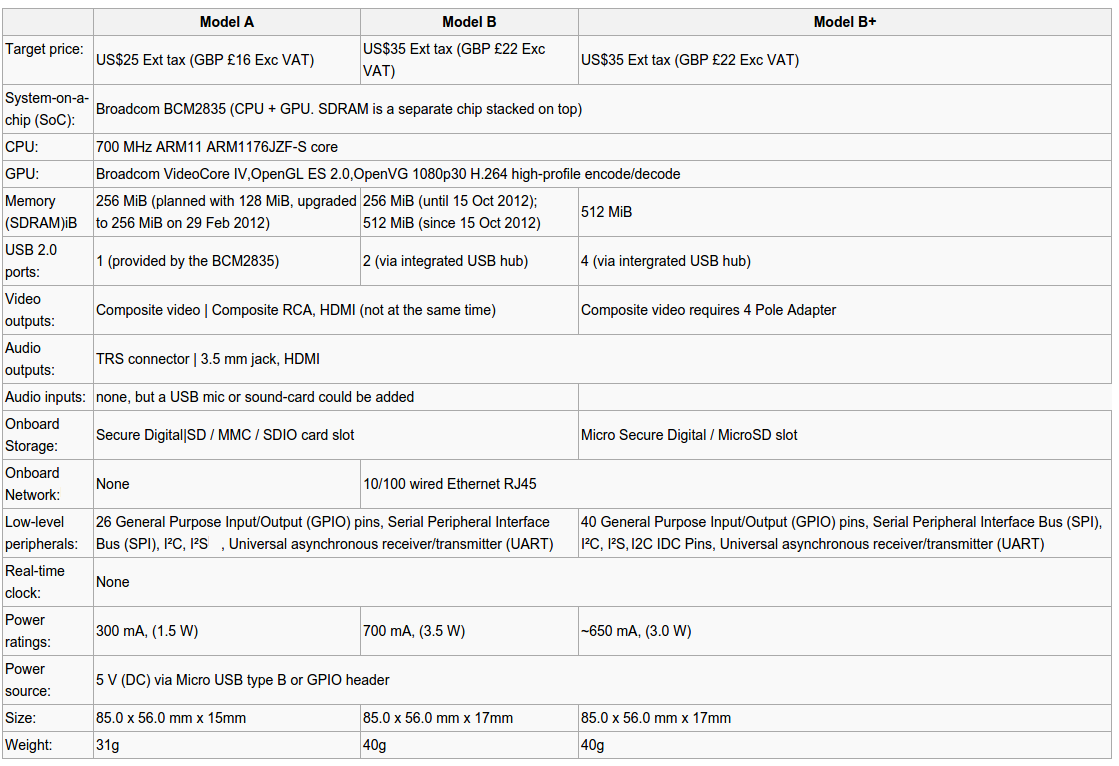
\includegraphics[width=1.0\textwidth,natwidth=610,natheight=642]{pictures/modelSpecification.png}
	\caption[Caption for LOF]{Models and Specifications\protect\footnotemark}    
    \label{fig:modelSpec}
\end{figure}
\footnotetext{\url{http://en.wikipedia.org/wiki/Raspberry_Pi}}


\balancecolumns
% That's all folks!

\end{document}
